\ProvidesClass{pom_thesis}[1/16/15]
\documentclass{pom_thesis}

\usepackage[utf8]{inputenc}
\usepackage{amsmath}
\usepackage{xcolor}
\usepackage{amssymb}
\usepackage{mathtools}
\usepackage[english]{babel}
\usepackage{hyperref}
\usepackage{multicol}
\usepackage{enumitem}
\usepackage{array}
\newcolumntype{P}[1]{>{\centering\arraybackslash}p{#1}}
\newcolumntype{M}[1]{>{\centering\arraybackslash}m{#1}}
\usepackage{cite}
\usepackage{listings}
\usepackage{csquotes}
\usepackage{subfig}
\usepackage{color} %red, green, blue, yellow, cyan, magenta, black, white
\definecolor{mygreen}{RGB}{28,172,0} % color values Red, Green, Blue
\definecolor{mylilas}{RGB}{170,55,241}
\usepackage[toc,page]{appendix}
\newcommand{\comment}[1]{}


\title{Kalman Filter Methods for Model Parametrization}

\author{Lindsey Tam }
\advisor{Blerta Shtylla}

\begin{document}

\maketitle

\begin{abstract}
	This thesis explores the theory and applications of Kalman Filters in both state and parameter estimation. Kalman Filters recursively generate predictions for linear dynamical systems and these predictions become progressively more accurate because of the system's ability to correct predictions using incoming data. Kalman Filters have many applications and in this thesis, we explore different Kalman Filters in order to fit ordinary differential equations models to data. Nonlinear forms of the Kalman Filter exist, including the Extended Kalman Filter (EKF) and the Unscented Kalman Filter (UKF). The EKF works by linearizing the system around the mean, making it more effective for simpler and lower dimensional systems. The UKF addresses the shortcomings of the EKF by linearizing the system around multiple points, known as sigma points. After exploring the theory behind these techniques, this thesis implements a few examples of the EKF and the UKF for both state and parameter estimation. \end{abstract}

\pagenumbering{roman}
\tableofcontents


\chapter{Introduction}
\label{Introduction}

\noindent This thesis explores the theory and computational implementation of the Kalman Filter (KF), Extended Kalman Filter (EKF), and the Unscented Kalman Filter (UKF). The KF is a data assimilation method that estimates the value of states in linear dynamical systems. Beyond state estimation, the KF can also be used for parameter estimation. The method of parameter estimation explored in this thesis is known as joint parameter estimation and involves creating new states for the estimated parameters.\\ 

\noindent Chapter 2 introduces state space models and methods of discretization, which are important foundations for implementing the KF. The two methods of discretization include using the matrix exponential and Euler's method. Included in this chapter is a brief example that demonstrates how to put a system into its state space format. \\ 

\noindent Chapter 3 explores the theory and algorithm of the KF. The KF is a recursive predictive-corrective process that enables the continuous generation of predictions about state variables without relying on large amounts of initial data. Applications of the KF include navigation and mage processing. \\ 

\noindent In the case of nonlinear dynamical systems, alternative forms of the Kalman Filter were developed, including the EKF and the UKF. Chapter 4 explains the theory of the EKF and its ability to linearize the system around the mean by taking the Jacobian of the nonlinear function. Navigation and signal processing are the main applications of the EKF. This chapter also implements an example of the EKF in both state and parameter estimation using a biological system that models metabolites. \\

\noindent Chapter 5 discusses the theory of the UKF. Instead of linearizing the system around a single point, the UKF utilizes many points. Applications of the UKF includes parameterization of math models in biology. This chapter also implements two examples of the UKF: state estimation of the Van der Pol oscillator as well as state and parameter estimation in the same metabolites example from Chapter 4.  \\ 

\noindent The ultimate goal of researching the UKF is to create a model that can forecast glucose values in real time of patients with Type 1 diabetes. Chapter 6 discusses how using the UKF for parameter estimation can be applied to an existing 12 state model for Type 1 Diabetes. Implementing this model has the potential to improve treatment methods and the quality of life of Type 1 diabetes patients.


\comment{
\noindent In the case of nonlinear dynamical systems, alternative forms of the Kalman Filter were developed, including the EKF and the UKF. The EKF linearizes the nonlinear system around the mean by taking the Jacobian of the nonlinear function. Navigation and signal processing are the main applications of the EKF. Instead of linearizing the system around a single point, the UKF utilizes many points. Applications of the UKF includes parameterization of math models in biology. Beyond state estimation, these filters can also be used for parameter estimation. The method of parameter estimation explored in this thesis is known as joint parameter estimation and involves creating new states for the estimated parameters. \\ 

\noindent In addition to understanding the theory behind these algorithms, this thesis also explores how they can be applied to real world systems. The first example observes a system that models the pathway of human metabolites, which are the byproducts of the metabolism. The goal of this example is to understand how the EKF works, how it can be used for multiple state correction, and how parameter estimation can be applied. A second example explored in this paper involves applying the UKF to the Van der Pol oscillator, which is a self sustaining nonconservative oscillator. The purpose of this simple example is to demonstrate how a simple version of UKF can be implemented on MATLAB while also observing how process and measurement noise influences the system. The third and final example uses the same metabolites system as the first example, but applies it in the context of the UKF. The parameter estimation results from the EKF and UKF on the metabolites system, are both promising. Though performance of the two is similar, the UKF can be further optimized by adjusting the model's hyper-parameters, which the EKF does not have. \\ 

\noindent  The ultimate goal of researching the UKF is to create a model that can forecast glucose values in real time of patients with Type 1 diabetes. This is inspired by a separate study that was able to do real-time glucose forecasting in Type 2 diabetes patients. Using an existing model of Type 1 diabetes that includes 12 states, the UKF will be most useful in extracting parameter values. Implementing this model has the potential to improve treatment methods and the quality of life of Type 1 diabetes patients.
}






\chapter{State Space Models}
\label{State Space Models}


Applying the Kalman Filter to a system requires an understanding of state space models. A state space model represents a system's inputs, outputs, and states by describing a series of first order differential equations. A linear continuous state space system has a general form of 
\begin{align*}
&\dot x(t)= A x(t) + B u(t) +w(t) \quad &\text{(system)}, \\
&y(t) = H x(t) +v(t) \quad &\text{(observation)} ,
\end{align*}
where $x$ is the state vector, $A$ is a square transformation matrix, $B$ is the input matrix, $u$ is a system input, $w$ is the process noise vector, $y$ is the transformed prediction, $H$ is the observation matrix, $v$ is the measurement noise vector, and $t$ is time. \\

\noindent For implementing Kalman Filters, the continuous state space system must be discretized into time steps, call it $k$. The general equation is given below as
\begin{align*}
& x_k= e^{At}x_{k-1} + \int_0^t e^{A(t-r))} B u_k dr + w_k \quad &\text{(system)}, \\
&y_k = H x_k + v_k  &\text{   (observation)} ,
\end{align*}
where $e^{At}$ is the matrix exponential of $A$. Generally, the matrix exponential is very time-consuming to compute, especially if the matrix is not diagnolizable. In these cases, an alternative solution is to use Euler's method, which approximates the discretized system using small time steps, as shown by 
\begin{align*}
& x_k= x_{k-1} + t f(x) &\text{(system)}, \\
&y_k = H x_k + v_k  &\text{(observation)},
\end{align*}
where $t$ is some small time step and $f(x)$ is the state after it undergoes a transformation. In most of the examples that are explored in this thesis, computing the matrix exponential is inefficient and results in excessive computing time. Therefore, Euler's method will be mostly used for discretization.

\noindent Consider an example of a moving mass, call it $m$, under a force, call it $u(t)$. The goal of this system is to predict the mass's position and velocity given its previous position and velocity. Therefore, position and velocity are the two states in this system. From differential equations, recall that the position of the mass is denoted by $x(t)$, the velocity of the mass is denoted by $\dot{x}(t)$, and the acceleration is denoted by $\ddot{x}(t)$. According to Newton's second law of motion, the force exerted on an object is given by the equation $F=ma$, or
\begin{align*}
u(t)=m\ddot{x}(t).
\end{align*}

\noindent This is a second order differential equation. To convert it into its state space format, begin by transforming it into a first order differential equation by substituting $x_1(t)$ for $x(t)$ and $x_2(t)$ for $\dot{x}(t)$, resulting in
\begin{align*}
\dot{x}_1(t) = x_2(t), \\
\dot{x}_2(t) = \frac{u(t)}{m}.
\end{align*}

\noindent For the sake of simplicity, assume this system has no process or measurement noise. The state vector, $x$, containing both position and velocity, can now be rewritten as
$$
x=
\begin{bmatrix}
x_1(t)\\
x_2(t)
\end{bmatrix}.
$$

\noindent In order to predict the state of the system at the next time step, take the derivative of the state vector and rewrite it in vector-matrix form (which is possible because this system is linear), resulting in
$$
\dot x=
\begin{bmatrix}
\dot{x}_1(t)\\
\dot{x}_2(t)
\end{bmatrix}=
\begin{bmatrix}
x_2(t)\\
\frac{u(t)}{m}
\end{bmatrix}=
\begin{bmatrix}
0 & 1\\
0 & 0
\end{bmatrix} x +
\begin{bmatrix}
0\\
\frac{1}{m}
\end{bmatrix} u(t).
$$
Here, one can see how this form can be applied to the general linear state space model where $A = 
\begin{bsmallmatrix}
0 & 1\\
0 & 0
\end{bsmallmatrix} $ and $ B=[0, \frac{1}{m}]^T$. \\

\noindent For the sake of this example, assume that only the position of the mass is measurable. Therefore, the transformed prediction, $y$, is given by
$$
 y=
\begin{bmatrix}
x_1(t)\\
0
\end{bmatrix}=
\begin{bmatrix}
1 \\
0
\end{bmatrix} x=
x_1(t). $$

\noindent Now that the continuous state system is defined, it can be discretized. Since this example considers a simple linear system, the matrix exponential can be calculated as follows 

$$e^{At} =
\begin{bmatrix}
e^0& e^t \\
0 & e^0
\end{bmatrix}=
\begin{bmatrix}
1& t\\
0 & 1
\end{bmatrix},
$$

$$\int_0^t e^{A(t-r))}  e^{At} B u_k dr=
\int_0^t e^{A(t-r))}  \begin{bmatrix}
1& t\\
0 & 1
\end{bmatrix} 
\begin{bmatrix}
0\\
\frac{1}{m}
\end{bmatrix} u(t) dt =
\int_0^t e^{A(t-r))}   \begin{bmatrix}
\frac{t}{m}\\
\frac{1}{m} 
\end{bmatrix} u(t) dt =
\begin{bmatrix}
\frac{t^2}{2m}\\
\frac{t}{m}
\end{bmatrix} u(t).
$$
Now the discretized state space model can be written as 


\begin{align*}
x &=
\begin{bmatrix}
1& t\\
0 & 1
\end{bmatrix}+x_{k-1}
\begin{bmatrix}
\frac{t^2}{2m}\\
\frac{t}{m}
\end{bmatrix} u(t) &\text{(system)}, \\
y &=
\begin{bmatrix}
1 \\
0
\end{bmatrix} x &\text{(observation)}.
\end{align*} \\

\noindent It is important to be able to discretize state space models because the goal of the Kalman Filter is to make some prediction about a future state. Therefore, discretization enables the Kalman Filter to make approximations about the system's state given past information. In addition, discretization makes numerical computing more efficient.


























\chapter{Kalman Filters}
\label{Kalman Filters}



The Kalman Filter (KF) recursively generates predictions for linear dynamical systems \cite{inbook}. The basic foundations of the this algorithm include generating a prediction given some initial knowledge of the data and using actual measurements from the system to continually correct the prediction. Therefore,  unlike other predictive methods like machine learning, the KF can begin generating estimates without large amounts of initial data. The KF begins by assuming the given data is noisy and Gaussian \cite{inproceedings, article7}. The first predictive step assumes knowledge of initial states and the model process. Since we know the system is linear, the model process can be denoted as a matrix and the states can be expressed as a vector. Through matrix vector  multiplication, this algorithm simulates how states are transformed after undergoing some process. The next step involves calculating the covariance in order to calculate the Kalman Gain, which is a measure of how much the estimate should be changed given actual measurements of the system. The corrective step utilizes the Kalman Gain, which is a measure of trust in either the measurements or the model, and the system measurements to gauge whether to depend more on the model or on the data. This process can be done recursively, allowing the model to become progressively more accurate as more data is added. Therefore, overtime, it is expected that the model will converge with the actual system measurements.
\\  \\

\begin{figure}[h]
    \centering
    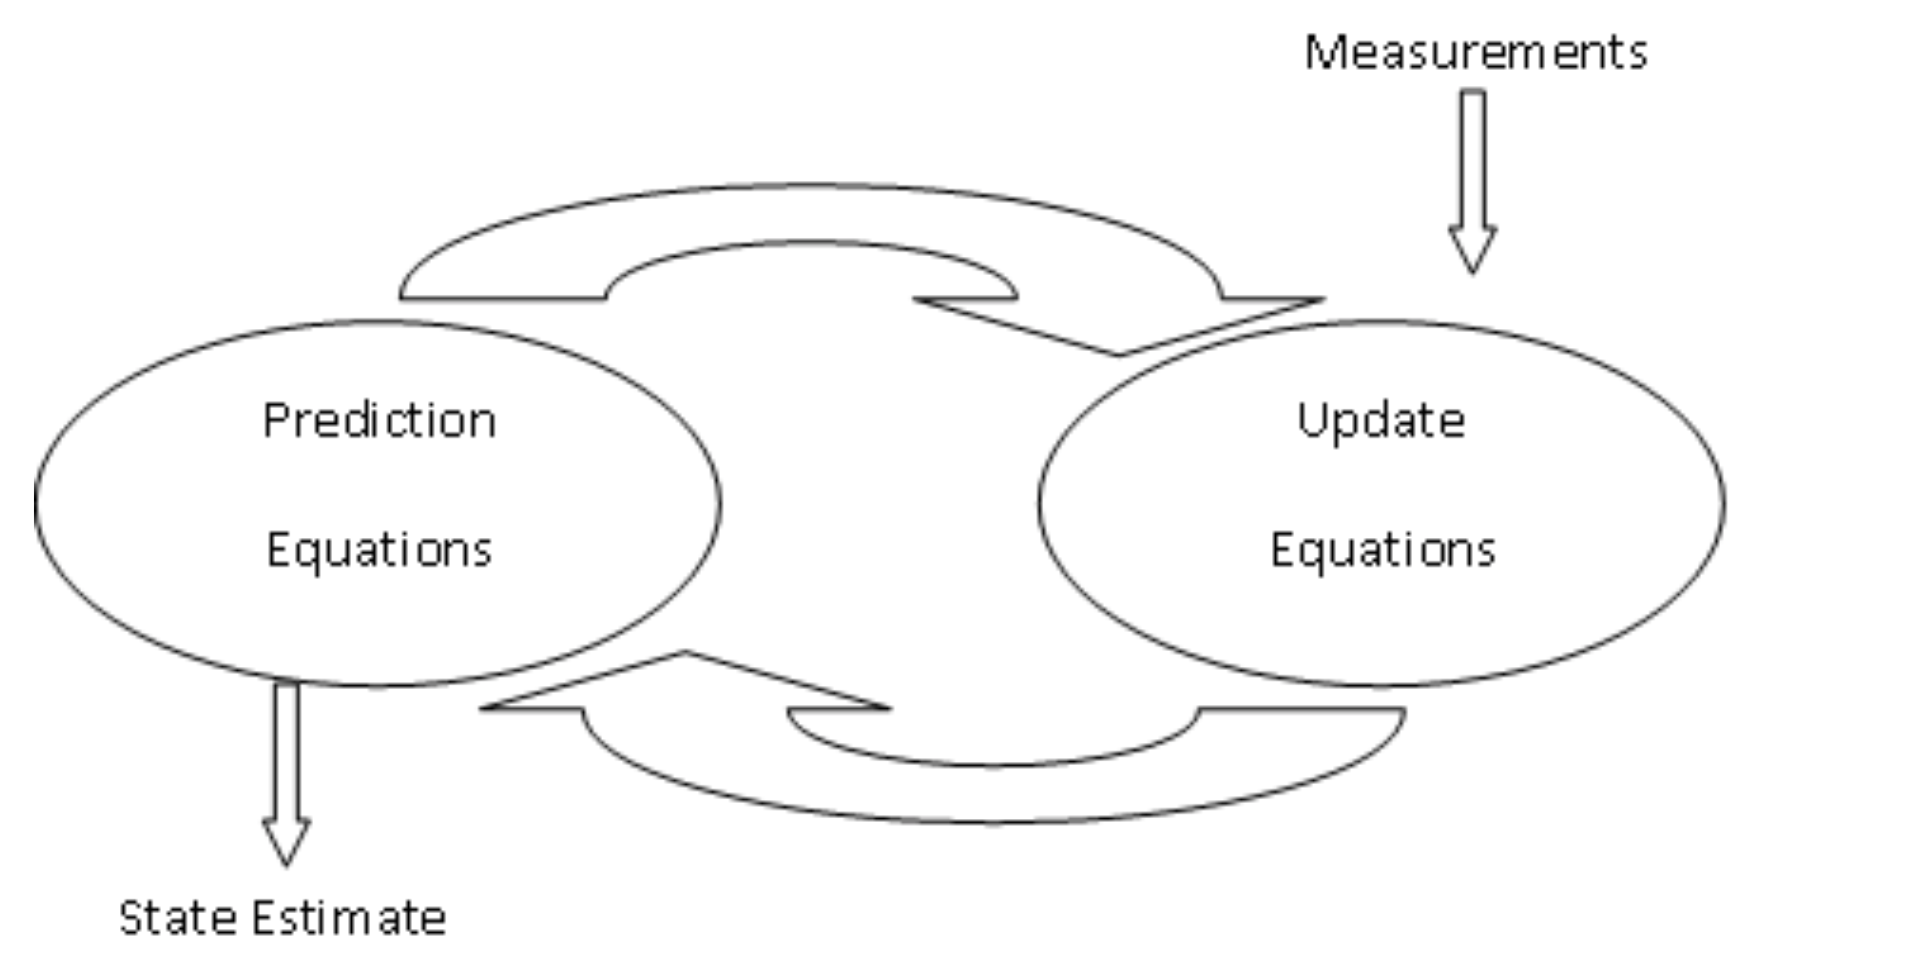
\includegraphics[scale = 0.3]{diagram.png}
    \caption{A basic diagram of the recursive nature of the Kalman Filter \cite{kohanbash_2014}.}
\end{figure}
\newpage


\begin{figure}[h]
    \centering
    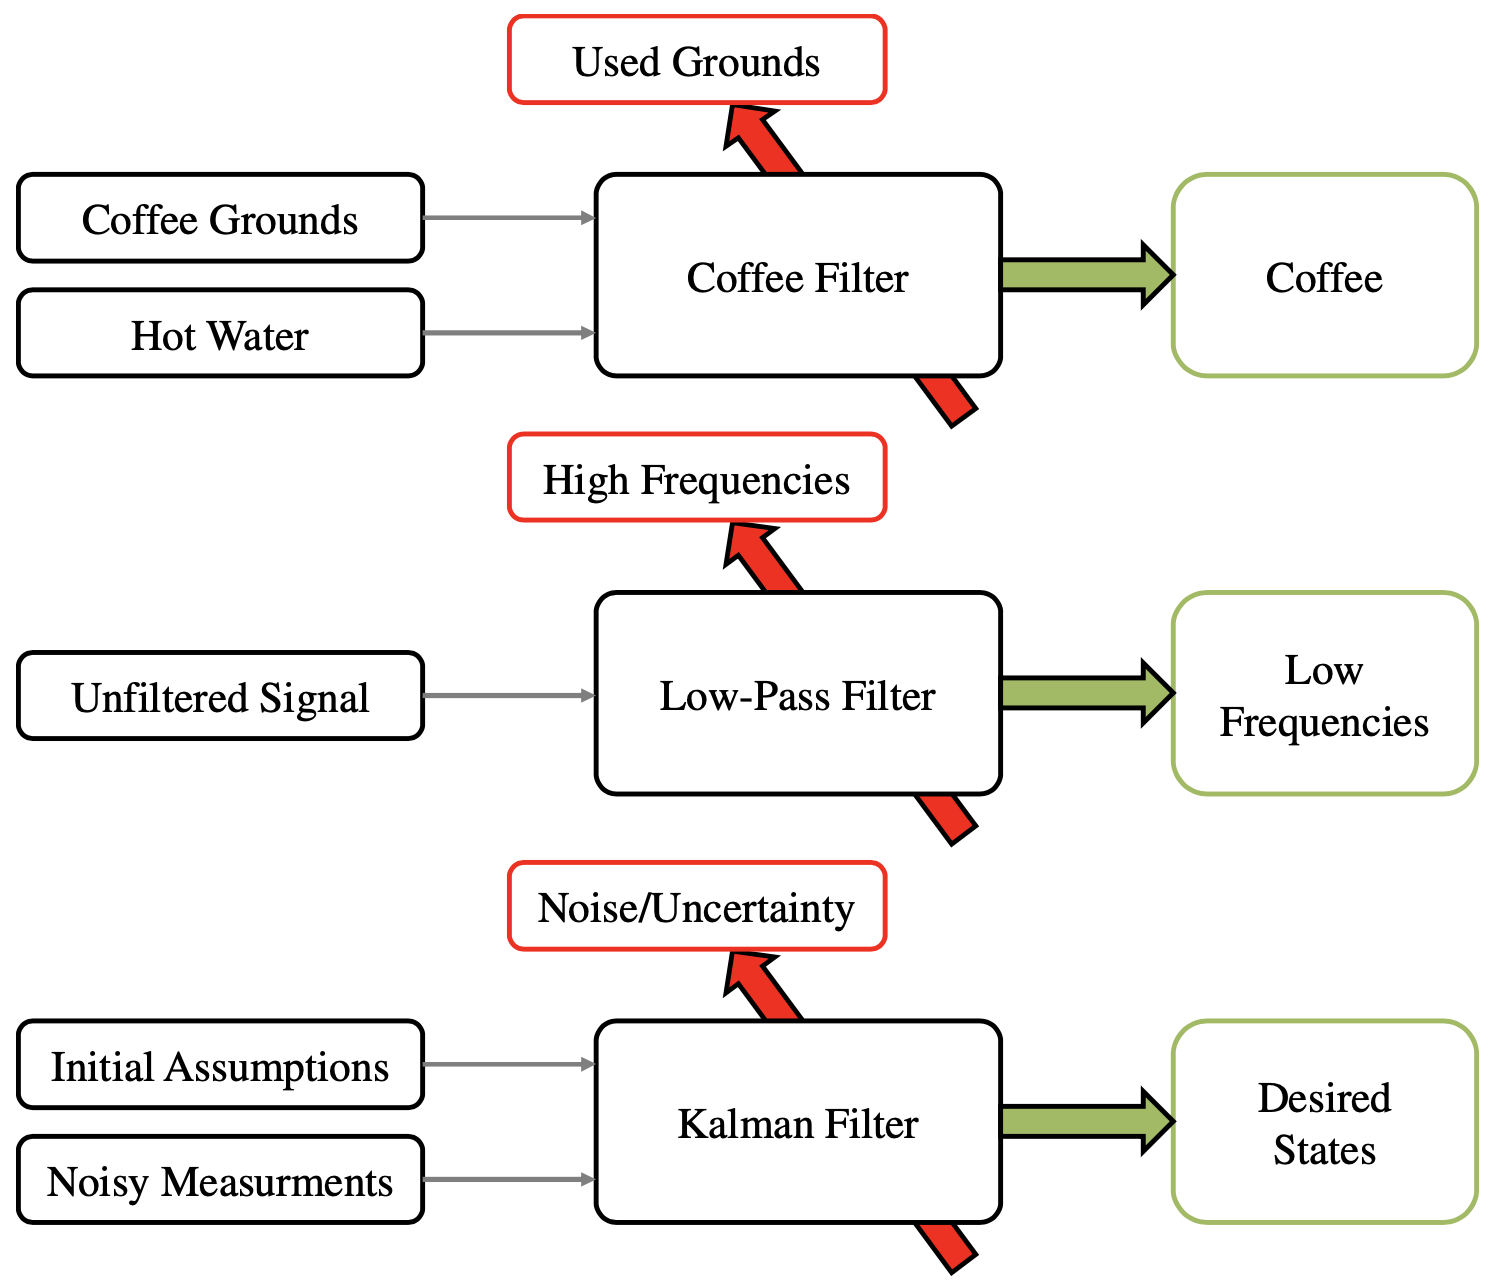
\includegraphics[scale = 0.3]{coffee.png}
    \caption{A simpler way to explore the KF is to facilitate a comparison with a coffee filter. This image is taken from a paper by Rhudy et al. comparing the Kalman Filter to a coffee filter \cite{article7}.}
    \end{figure}

\newpage

\noindent The most common application of KFs is in navigation, image processing, and finance. A relevant example is using computer vision to monitor and track vehicles in real time. Another example is the development of the Global Positioning Systems (GPS) \cite{lim_ong_lim_koo_2016}. The KF also has many aeronautical applications, which include long-distance flight,  and autopilot systems. In fact, the KF was created to development the navigation system in the Apollo Program \cite{kalmanbio}.  \\ \\


\noindent The Kalman Filter is named after its developer, Rudolph Emil Kalman. Kalman was born on May 19, 1930 in Budapest, Hungary. After arriving in the United States, Kalman completed his undergraduate studies and masters degree in electrical engineering from Massachusetts Institute of Technology and completed his doctoral degree in Columbia University. He would spend the next years of his life teaching. In the 1960s to 1970s he became a professor at Stanford university \cite{kalmanbio}. In the 1970s and 1990s, Kalman spent time as professor of  engineering at the University of Florida. Kalman is most known for his work on the Kalman Filter, which was developed in the late 1950s. The Kalman Filter greatly aided the United States' military projects, resulting in former President Obama to award Kalman the National Medal of Science in 2009. In addition, in 1985, Kalman was awarded the Kyoto Prize, which is the Japanese version of the Nobel Peace Prize. Kalman passed away July 2, 2016 at the age of 86 and is survived by his wife and two children \cite{Kalman_bio}. 


\newpage

\section{Kalman Filter Algorithm}

Before  delving into the formal steps of the Kalman Filter, it is important to understand the underlying foundation of this method. 
\noindent The goal of the Kalman Filter is to predict the new state of a system, after it undergoes some transformation. Let this be represented by 
\begin{align*}
	\frac{dx}{dt} = f(x) + \varepsilon ',
\end{align*}
where $\frac{dx}{dt}$ is the prediction of the states, $f(x)$ is a function that transforms the states, and $ \varepsilon '$ is internal system noise. Assuming we have some understanding of the system, we can represent this transformation using matrix $M'$ to approximate the equation above as
\begin{align*}
	\frac{dx}{dt} \approx M'x + \varepsilon '.
\end{align*}

\noindent The Kalman Filter works by generating predictions and making correction at various time steps. Let these time steps be denoted as $k$, such that $ k $ is a nonnegative integer and let $x_k$ be the estimate of the state variables at time $k$ with initial assumptions of the state variables beginning at $x_0$ such that $x_0 = \mathcal{N}(m_0, c_0) $. 

\begin{figure}[h]
    \centering
    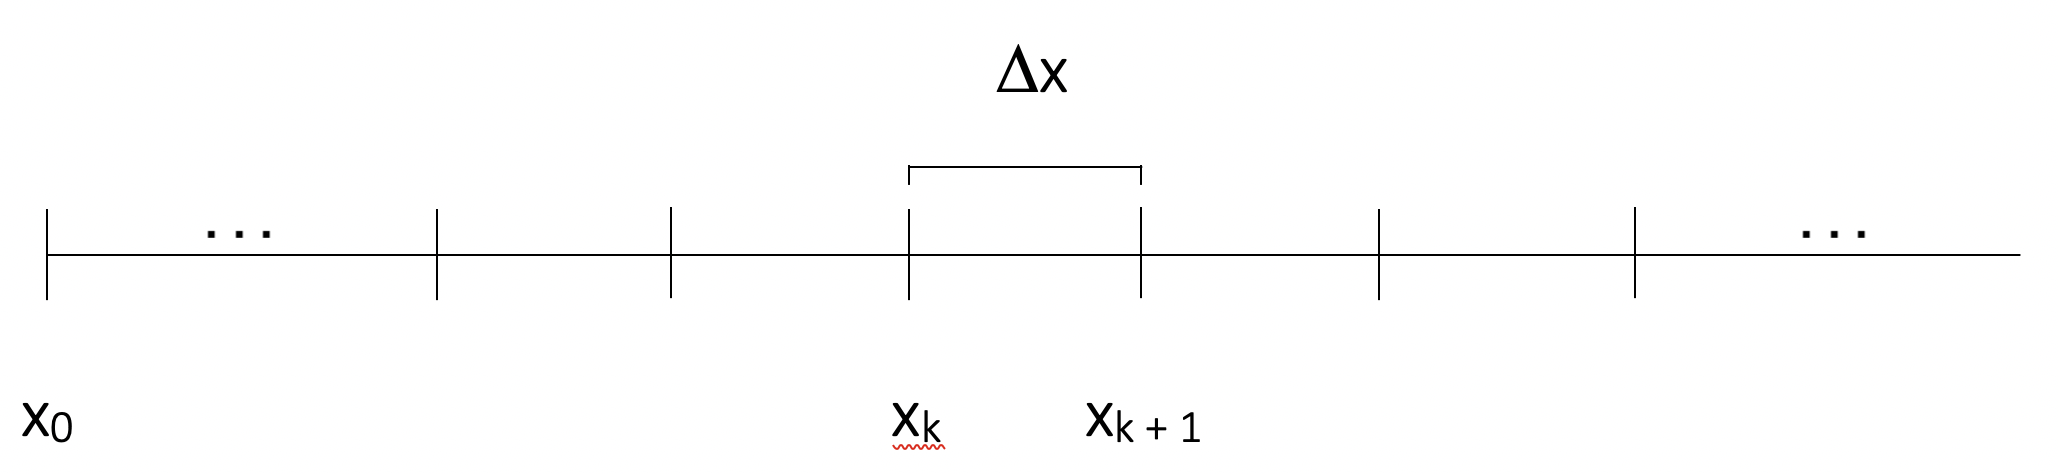
\includegraphics[scale = 0.3]{kgraph.png}
    \caption{A diagram showing discretized time steps of a system. Though this diagram depicts time steps that are equal, this should not be assumed for all cases.}
\end{figure}

\noindent Next, approximate $\frac{dx}{dt}$ using the limit definition of derivative:
\begin{align*}
	\frac{x_{k+1} - x_k}{\Delta t} \approx M'x_k + \varepsilon '_k \\
	x_{k+1} - x_k \approx M'x_k \Delta t + \varepsilon '_k  \Delta t \\
	x_{k+1} \approx M'x_k \Delta t + \varepsilon '_k  \Delta t + x_k \\
	x_{k+1} \approx (M' \Delta t + I)x_k + \varepsilon '_k  \Delta t
\end{align*}


\noindent From here, substitute $M$ for $M' \Delta t + I$ and $\varepsilon_k$ for  $\varepsilon '_k  \Delta t $ to get
\begin{align*}
	x_{k+1} \approx M x_k + \varepsilon_k,
\end{align*}
\noindent where $\varepsilon_k = \mathcal{N}(0, c_1)$. This general equation is significant to the generation of predictions and will continue to be used in different versions of the Kalman Filter. \\ 

\noindent Another important aspect of the KF is the incorporation of state measurements. The estimate of the the system measurement at the next time step, call it $y_{k+1}$, is given by 
\begin{align*}
	y_{k+1} \approx H x_{k+1} + v_{k+1},
\end{align*}
where $H_k$ is the observation function and $v_k$ is measurement noise such that $v_k = \mathcal{N}(0, c_2)$. \\


\begin{enumerate}
  \item Begin by initializing the state estimate and the initial state covariance matrix. The state estimate, $x_0$,  is a  column vector containing state variables, call them $x_a, x_b, \hdots, x_n$, such that $x_0= [x_a, x_b, \hdots, x_n]^T$, where $T$ is the transpose. The stat estimate can be found by taking the expected value of the data where data is normally distributed. If the system states are finite, the expectation is denoted by
    \begin{align*}
        \mathbb{E}[x_0]   = \sum^n_{i = a} x_i p_i = [x_a p_a + x_b p_b + \hdots + x_n p_n]^T,
        %= \begin{bmatrix}
          % x_a \\
           %\vdots \\
           %x_ 
        % \end{bmatrix}.
    \end{align*}
    
    $p_a, p_b, \hdots, p_n$ is the respective probability of getting each state variable.    The state covariance matrix, $P_0$, is a square matrix whose contents are the covariance of the pairwise elements
    \footnote{Recall that the covariance of a variable with itself is the variance of the variable}
    , or
    \begin{align*}
      P_0 =
      \begin{bmatrix}
           var(x_a)  & \hdots & cov(x_a,x_n) \\
           \vdots & \ddots & \vdots \\
           cov(x_n, x_a)  & \hdots & var(x_n )
         \end{bmatrix} .
  \end{align*}
  Enough should be known about the modeled system to generate these values. In general, $\hat x_k$ denotes the model's estimate of the state variables. When initializing these values, we use $x_0$, which is the actual initial measurements of the system. \\ \\
   A state covariance matrix is a symmetrical positive semi-definite square matrix whose diagonals correspond to the variance of a variable at location i and elsewhere is the covariance of the pairwise elements. In practice, covariance matrices help us better understand the spread of data. For the case of the KF, calculating the state covariance is necessary for computing Kalman Gain. 
   
   
  \item After initializing the state estimate and state covariance, a prediction can be generated. The estimate of the system at the next time step, $x_{k+1}$,  is given by
  \begin{align*}
      x_{k+1} = F x_{k} +  G u_{k} + w_{k} ,
  \end{align*} 
  where $F$ is the state matrix, $G$ is the F and input matrix, $u_k$ is an input vector and $w_k$ is the process noise vector. Every state variable contained in $x_k$ is defined by a linear differential equation. These linear differential equations can be used to generate the F and G matrices. Therefore, F should be a square matrix whose dimension is equal to the number of states variables and G can be a matrix (or in some cases a vector), depending on the dimension of input vector u. \\ \\
  $u_k$  is an input vector, which is a measurable value that helps define the system, but is not contained in the state vector. Depending on how the system is defined, $u_k$  can be a constant value or it can be a value dependent on time step k. \\ \\
  $w_k$ is the process noise vector at time k. Process noise can be thought of as the model's accuracy. When process noise is 0, it implies that the model is perfectly accurate and does not have to correct for incoming system measurements. On the other hand, high process noise will essentially restate the system based on incoming measurements. $w_k$ has the same dimensions as $x_k$, allowing us to identify whether or not to adjust the equations for the state variables. When all values of  $w_k$ equal 0, it implies that the linear differential equations we are using to define the state variables have no error. 
  
  
  
  \item Next, the state covariance matrix to calculate Kalman Gain. The state covariance matrix at time step $k$ given the last time step, is 
    \begin{align*} 
        P_{k | k -1} = F P_{k - 1} F^T + Q_{k-1}, 
    \end{align*}
    where $F^T$ is the transpose of $F$, and $Q_{k}$ is the process noise covariance of $w_k$.
    The Kalman Gain at time step $k$, is given by
    \begin{align*} 
        K_k = P_{k | k - 1} H^T_K (H_k P_{k | k - 1} H^T_K + R_k)^{-1},
    \end{align*}
      where $H$ is the observation matrix and $R$ is measurement noise covariance. 
      $H$ enables the state variables to be linearly transformed to match the outputs of the system. The dimensions of $H$ reflects which state variables have measurable values in the system. It is not assumed that every state variable is measurable, so $H$ allows us to compare the measurable state variables to $x_k$. Simple applications of $H$ include creating matrices with 0's and 1's, with 1's denoting that a state variable is measurable and a 0's representing non-measurable states. In other cases, $H$ is an integer used as a scaling factor. \\ \\
     The Kalman Gain is the main component of the corrective aspect of the KF. The Kalman Gain is a measure of how much to change the model based on incoming data. Low values of the Kalman Gain imply the model is accurate while higher values indicate the model should adjust based on the incoming data.  \\ \\
     From this equation, one can see that balancing $Q$ and $R$ is critical for model performance. Larger values of $Q$ indicate higher modeling error, which leads to a higher Kalman Gain and increased model correction. On the other hand, large values of $R$ imply high measurement error, leading to a lower Kalman Gain and less model correction. 
     
   
    \item Next, calculate the transformed output vector and correct the prediction. The transformed output vector, $\hat y_k$, is given by
    \begin{align*}
        \hat y_k = H_k x_k + v_k,
    \end{align*}
    
    where $v_k$ is measurement noise, which is added to account for measurement error.
    The corrected prediction, $x_k$, is given by
    \begin{align*} 
        x_k = x_{k - 1} + K_k(y_k - \hat y_{k}),
    \end{align*}
   where  $y_k$ is the actual measurements of the system, $K_k$ is the Kalman Gain, and $x_{k-1}$ are the values of the state variable at the last time step. $\hat y_k$ is a way of transforming the prediction (using $H$) into a format that can be compared with $y_k$. Subtracting the actual measurements from the predicted measurements is necessary, because $y_k$ does not always contain measurements for all variables in state vector $x_k$. The quantity $y_k - \hat y_{k}$ is also known as measurement residual or innovation.  \\
   
     \item The final step is to update the state covariance matrix, $P_k $, through the equation
    \begin{align*} 
        P_k = (I - K_k H_k) P_{k | k-1},
    \end{align*}
    where $I$ is the identity matrix, $K_k$ is the Kalman Gain, $H_k$ is the obersevation function, and $P_{k|k-1}$ is the state covariance at time step $k$ given the last time step. $ P_k $ will be used in the next iteration of the filter.
\end{enumerate} 


\newpage

\begin{center}
\begin{table}
\centering
\caption{Description of all variables in the Kalman Filter} \label{tab:sometab}
\begin{tabular}{ |p{2cm}||p{5cm}|p{2cm}| }
    \hline
    \multicolumn{3}{|c|}{Variables in the Kalman Filter } \\ 
    \hline
    Variable & Description & Dimensions \\
    \hline
    x & State variables  & $d_x \times 1$ \\
    y & Output vector  & $d_y \times 1$ \\
    u & System inputs  & $d_u \times 1$\\
    v & Measurement noise & $d_y \times 1$\\
    w & Process noise & $d_x \times 1$\\
    F & State function  & $d_x \times d_x $  \\ 
    H & Observation function & $d_y \times d_x$\\
    G & Input function & $d_x \times d_u$\\
    K & Kalman Gain  & $d_x \times d_y$\\
    Q & Process noise covariance  & $d_x \times d_x$ \\
    R & Measurement noise covariance &  $d_y \times d_y$\\
    P & Covariance matrix & $d_x \times d_x $  \\ 
    
    \hline
\end{tabular}

\end{table}
\end{center} 

\newpage

\section{Assessing Model Performance}





\chapter{Extended Kalman Filters}
\label{Extended Kalman Filters}

The Extended Kalman Filter (EKF) is the non-linear version of the Kalman Filter. Though it can be used for non linear equations, it is important to note that it is not an optimal estimator. For the most part, the EKF Algorithm is nearly identical to the KF algorithm. The critical difference is in linearizing the state and observation function. The EKF uses the Jacobean to linearly approximate the non-linear function around the mean of the Gaussian distribution. Skipping this step would result in the transformed data being non-Gaussian; though taking the Jacobean enables the transformation to remain Gaussian, it is not exact, resulting in some generalization. Linear approximation through a single point also makes the EKF inefficient when dealing with complex, higher order systems. Because of this, the model is highly subject to error, which can be somewhat reduced by setting accurate initial values. Though these flaws exist, the EKF performs strongly with applications of real time spatial fields, including navigation and positioning systems.  \\ \\

\section{Extended Kalman Filter Algorithm}

\begin{center}
    
\centering
\begin{tabular}{ |p{2cm}||p{5cm}|p{2cm}| }
    \hline
    \multicolumn{3}{|c|}{Variables in the Extended Kalman Filter } \\ 
    \hline
    Variable & Description & Dimensions \\
    \hline
   x & State variables  & $d_x \times 1$ \\
    y & Output vector  & $d_y \times 1$ \\
    u & System inputs  & $d_u \times 1$\\
    v & Measurement noise & $d_y \times 1$\\
    w & Process noise & $d_x \times 1$\\
    f & None linear state function  & $d_x \times d_x $  \\ 
    F & State function  & $d_x \times d_x $  \\ 
    h & Non linear observation function & $d_y \times d_x$\\
    H & Linearized observation function & $d_y \times d_x$\\
    K & Kalman Gain  & $d_x \times d_y$\\
    Q & Process noise covariance  & $d_x \times d_x$ \\
    R & Measurement noise covariance &  $d_y \times d_y$\\
    P & Covariance matrix & $d_x \times d_x $  \\ 
    \hline
\end{tabular}
\end{center}
\begin{enumerate}
  \item Initialize the state estimate ($x_0$) and the initial covariance matrix ($P_0$) 
  \begin{align*}
        \hat x_0 = \mathbb{E}[x_0]  = \begin{bmatrix}
           x_1 \\
           \vdots \\
           x_n 
         \end{bmatrix}  
    \end{align*}
  \begin{align*}
      P_0 =
      \begin{bmatrix}
           var(x_1)  & \hdots & cov(x_1, x_n) \\
           \vdots & \ddots & \vdots \\
           cov(x_n, x_1)  & \hdots & var(x_n )
         \end{bmatrix}  
  \end{align*}
  Often, $P_0 $ will be initialized as a diagonal matrix with the diaganals being the variance of each state variance and every other value being set to 0.
  \item Calculate the Jacobean
  \begin{align*}
      F= \frac{\partial f}{\partial x} =
      \begin{bmatrix}
           \frac{\partial f_1}{\partial x_1} & \hdots & \frac{\partial f_n}{\partial x_n} \\
           \vdots & \ddots & \vdots \\
           \frac{\partial f_n}{\partial x_1}  & \hdots & \frac{\partial f_n}{\partial x_n}
         \end{bmatrix}  
  \end{align*}
  \begin{align*}
      H = \frac{\partial h}{\partial x} =
     \begin{bmatrix}
           \frac{\partial h_1}{\partial x_1} & \hdots & \frac{\partial h_m}{\partial x_n} \\
           \vdots & \ddots & \vdots \\
           \frac{\partial h_m}{\partial x_1}  & \hdots & \frac{\partial h_{d_y}}{\partial x_n}
         \end{bmatrix}  
  \end{align*}
   Here, both $f$ and $h$ have no closed form solution. $f$ is the non-linear state function and $F$ is the linear approximation of $f$ with dimension $d_x$. Similarly, $h$ is the non linear observation while $H$ is linearized observation with dimension $d_y$. 
  \item Generate a prediction 
  \begin{align*}
      x_{k+1} = f( x_{k-1} , u_{k-1})  
  \end{align*} 
  This equation is different from the one used in the Kalman filter 
  \item Use the state covariance matrix ($P_{k | k - 1}$) to calculate Kalman Gain ($K_k$) 
    \begin{align*} 
        P_{k | k -1} = F P_{k - 1} F^T + Q_{k-1} 
        \end{align*}
         \begin{align*} 
        K_k = P_{k | k - 1} H^T_K (H_k P_{k | k - 1} H^T_K + R_k)^{-1}
    \end{align*}
    Recall that $H$ and $F$ are linear approximations of $f$ and $h$. Therefore, it is assumed that there is some amount of error when calculating the Kalman Gain.
    
    \item  Correct the prediction
    \begin{align*}
        \hat y_k = H( x_k + v_k )
    \end{align*}
     \begin{align*} 
        x_k = x_{k - 1} + K_k(y_k - \hat y_k)
    \end{align*}
    \item Update the covariance matrix
    \begin{align*} 
        P_k = (I - K_K H_k) P_{k | k-1}
    \end{align*}
\end{enumerate} 

\section{Modeling Metabolites using EKF}
\label{Modeling Metabolites using EKF}

\noindent This example is inspired by research that models the biological pathway of metabolites, which are molecules that are the byproduct of the body's metabolism. This model contains four different states, or metabolites, which contain 18 unknown parameters \cite{article5}. Unlike the original research, which had datasources of their own, this example will simulate data by using a built-in ODE solver on Matlab. Ultimately, the two goals of this example is to demonstrate how the EKF can be applied, how the EKF can correct for multiple variables or states, and how the EKF can be used for parameter fitting. \\ 

\noindent In this example, the four metabolites, or states, have the following differential equations:
\begin{align*}
\dot x_1 &= \alpha_1 x_3^{g_{13}} x_5^{g_{15}} - \beta_1 x_1^{h_{11}}, \\
\dot x_2 &= \alpha_2 x_1^{g_{21}} - \beta_2 x_2^{h_{22}}, \\
\dot x_3 &= \alpha_3 x_2^{g_{32}} - \beta_3 x_3^{h_{33}} x_4^{h_{34}}, \\
\dot x_4 &= \alpha_4  x_1^{g_{41}} - \beta_4 x_4^{h_{44}},
\end{align*}
where there are 18 unknown parameters ($\alpha_1, \hdots, \alpha_4, \beta_1, \hdots, \beta_4, g_{13}, g_{15}, g_{21}, \\ g_{32}, g_{41}, h_{11}, h_{22}, h_{33}, h_{34}, h_{44} $). Therefore, the state vector is given by $x_k = [x_{1,k}, x_{2,k}, x_{3,k}, x_{4,k}]^T$. We will use the EKF to find parameter values that best fit this model to its true states. In both the original example as well as this one, sampling time will be 0.1 seconds for 5 seconds, totaling 50 UKF estimates. Since we did not have access to the original example's dataset, data is simulated on MATLAB. Similar to the previous example, the system's true output was simulated using an ODE solver and incoming system measurements were calculated by adding noise to the true value. The model was initialized by setting the state variable to $x_0 = [4, 1, 3, 4]^T$ and the state covariance to $P_0 = .01I$. 

\subsubsection{Implementing EKF}

\noindent These states are given in a continuous state space model and need to be discretized. Recall that a continuous state space given by $\dot x(t) = Ax(t)$ can be discretized into $x_k = e^{At}x_{k-1}$. Here, our transition matrix, $A$, is not unique. One value for $A$, includes:
%\begin{align*}
%\dot x(t) = Ax(t)
%\end{align*}
$$
\scriptsize{
\begin{bmatrix}
-b1*x_1^{h_{11}-1} & 0 & x_5*x(3)^{g_{13}-1}& 0 & 0  & 0 & 0  & 0 \\
x_6*x(1)^{g_{21}-1} & -b2*x_2^{h_{22}-1}&0&0&0&0&0&0 \\
0&x_7*x_2^{g_{32}-1}&-b3*x_3^{h_{33}-1}*x_4^{h_{34}}&0&0&0&0&0\\
0&0&0&-b4*x_4^{h_{44}-1}&0&0&0&x_1^{g_{41}}\\
\end{bmatrix}}.
$$


\begin{figure}[h]
    \centering
    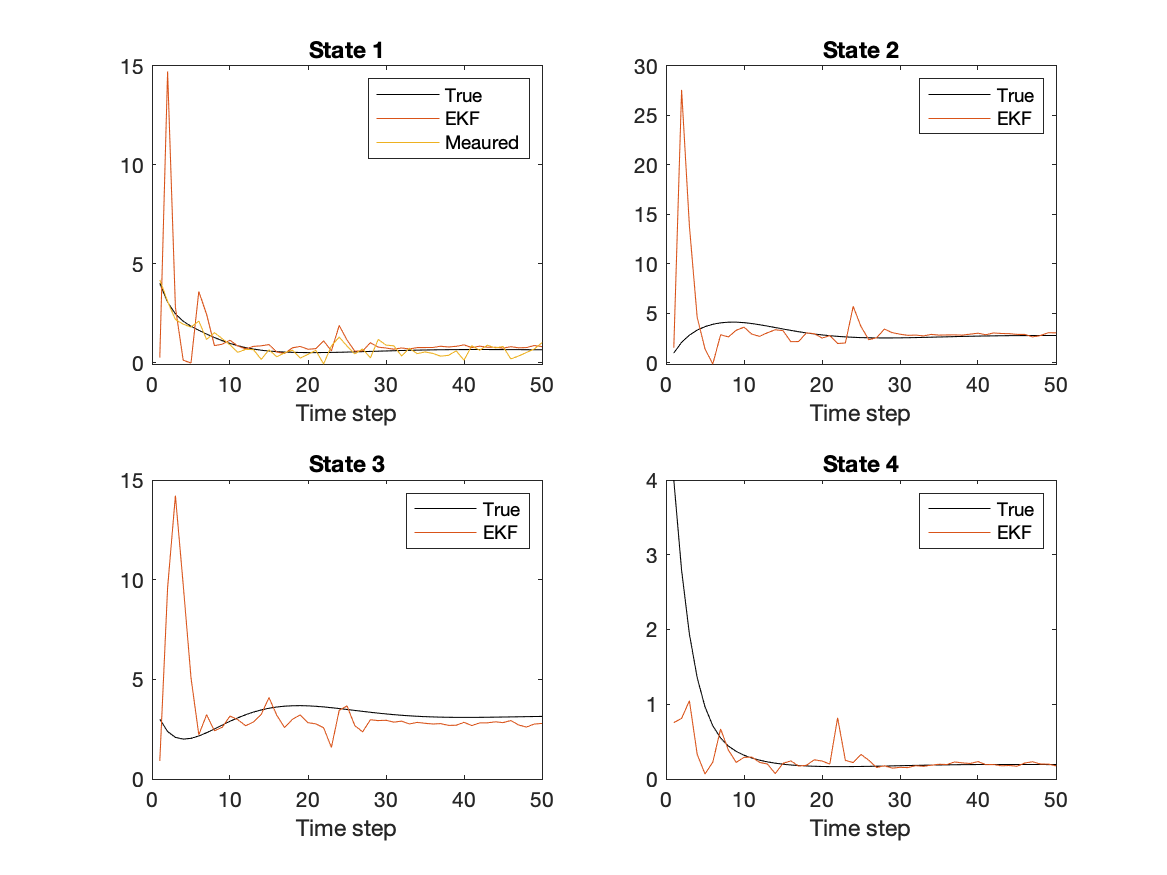
\includegraphics[scale = 0.6]{EKF_1_state.png}
    \caption{sdaasads}
\end{figure}

\subsubsection{EKF multiple state correction}

\subsubsection{EKF Parameter Estimation}

$$
\scriptsize{
\begin{bmatrix}
-b1*x_1^{h_{11}-1} & 0 & x_5*x(3)^{g_{13}-1}& 0 & 0  & 0 & 0  & 0 \\
x_6*x(1)^{g_{21}-1} & -b2*x_2^{h_{22}-1}&0&0&0&0&0&0 \\
0&x_7*x_2^{g_{32}-1}&-b3*x_3^{h_{33}-1}*x_4^{h_{34}}&0&0&0&0&0\\
0&0&0&-b4*x_4^{h_{44}-1}&0&0&0&x_1^{g_{41}}\\
0&0&0&0&0&0&0&0 \\
0&0&0&0&0&0&0&0 \\
0&0&0&0&0&0&0&0 \\
0&0&0&0&0&0&0&0 \\
\end{bmatrix}}.
$$
\begin{center}
\begin{table}

\caption{True Parameter Values} \label{tab:sometab}
\begin{tabular}{ |P{1cm}||P{1cm} P{1cm} P{1cm} P{1cm} P{1cm} P{1cm} P{1cm} P{1cm} P{1cm} P{1cm}|}
    \hline
    \multicolumn{11}{|c|}{True Parameter Values} \\ 
    \hline
      & $\alpha_i$ & $g_{i1}$ & $g_{i2}$ & $g_{i3}$ & $g_{i4}$ & $\beta_i$ & $h_{i1}$ & $h_{i2}$ & $h_{i3}$ & $h_{i4}$\\
    \hline
    $x_1$ & 20.0  & 0 & 0 & -0.8 & 0 & 10.0 & 0.5 & 0 & 0 & 0\\
    $x_2$ & 8.0  & .5  & 0 & 0 & 0 & 3.0 & 0 & 0.75 & 0 & 0\\
    $x_3$ & 3.0  & 0 & 0.75 & 0 & 0 & 5.0 & 0 & 0 & 0.5 & 0.2\\
    $x_4$ & 2.0 & .5  & 0 & 0 & 0 & 6.0 & 0 & 0 & 0 & 0.8\\
    
    \hline
\end{tabular}
\end{table}
\end{center}


\begin{figure}[h]
    \centering
    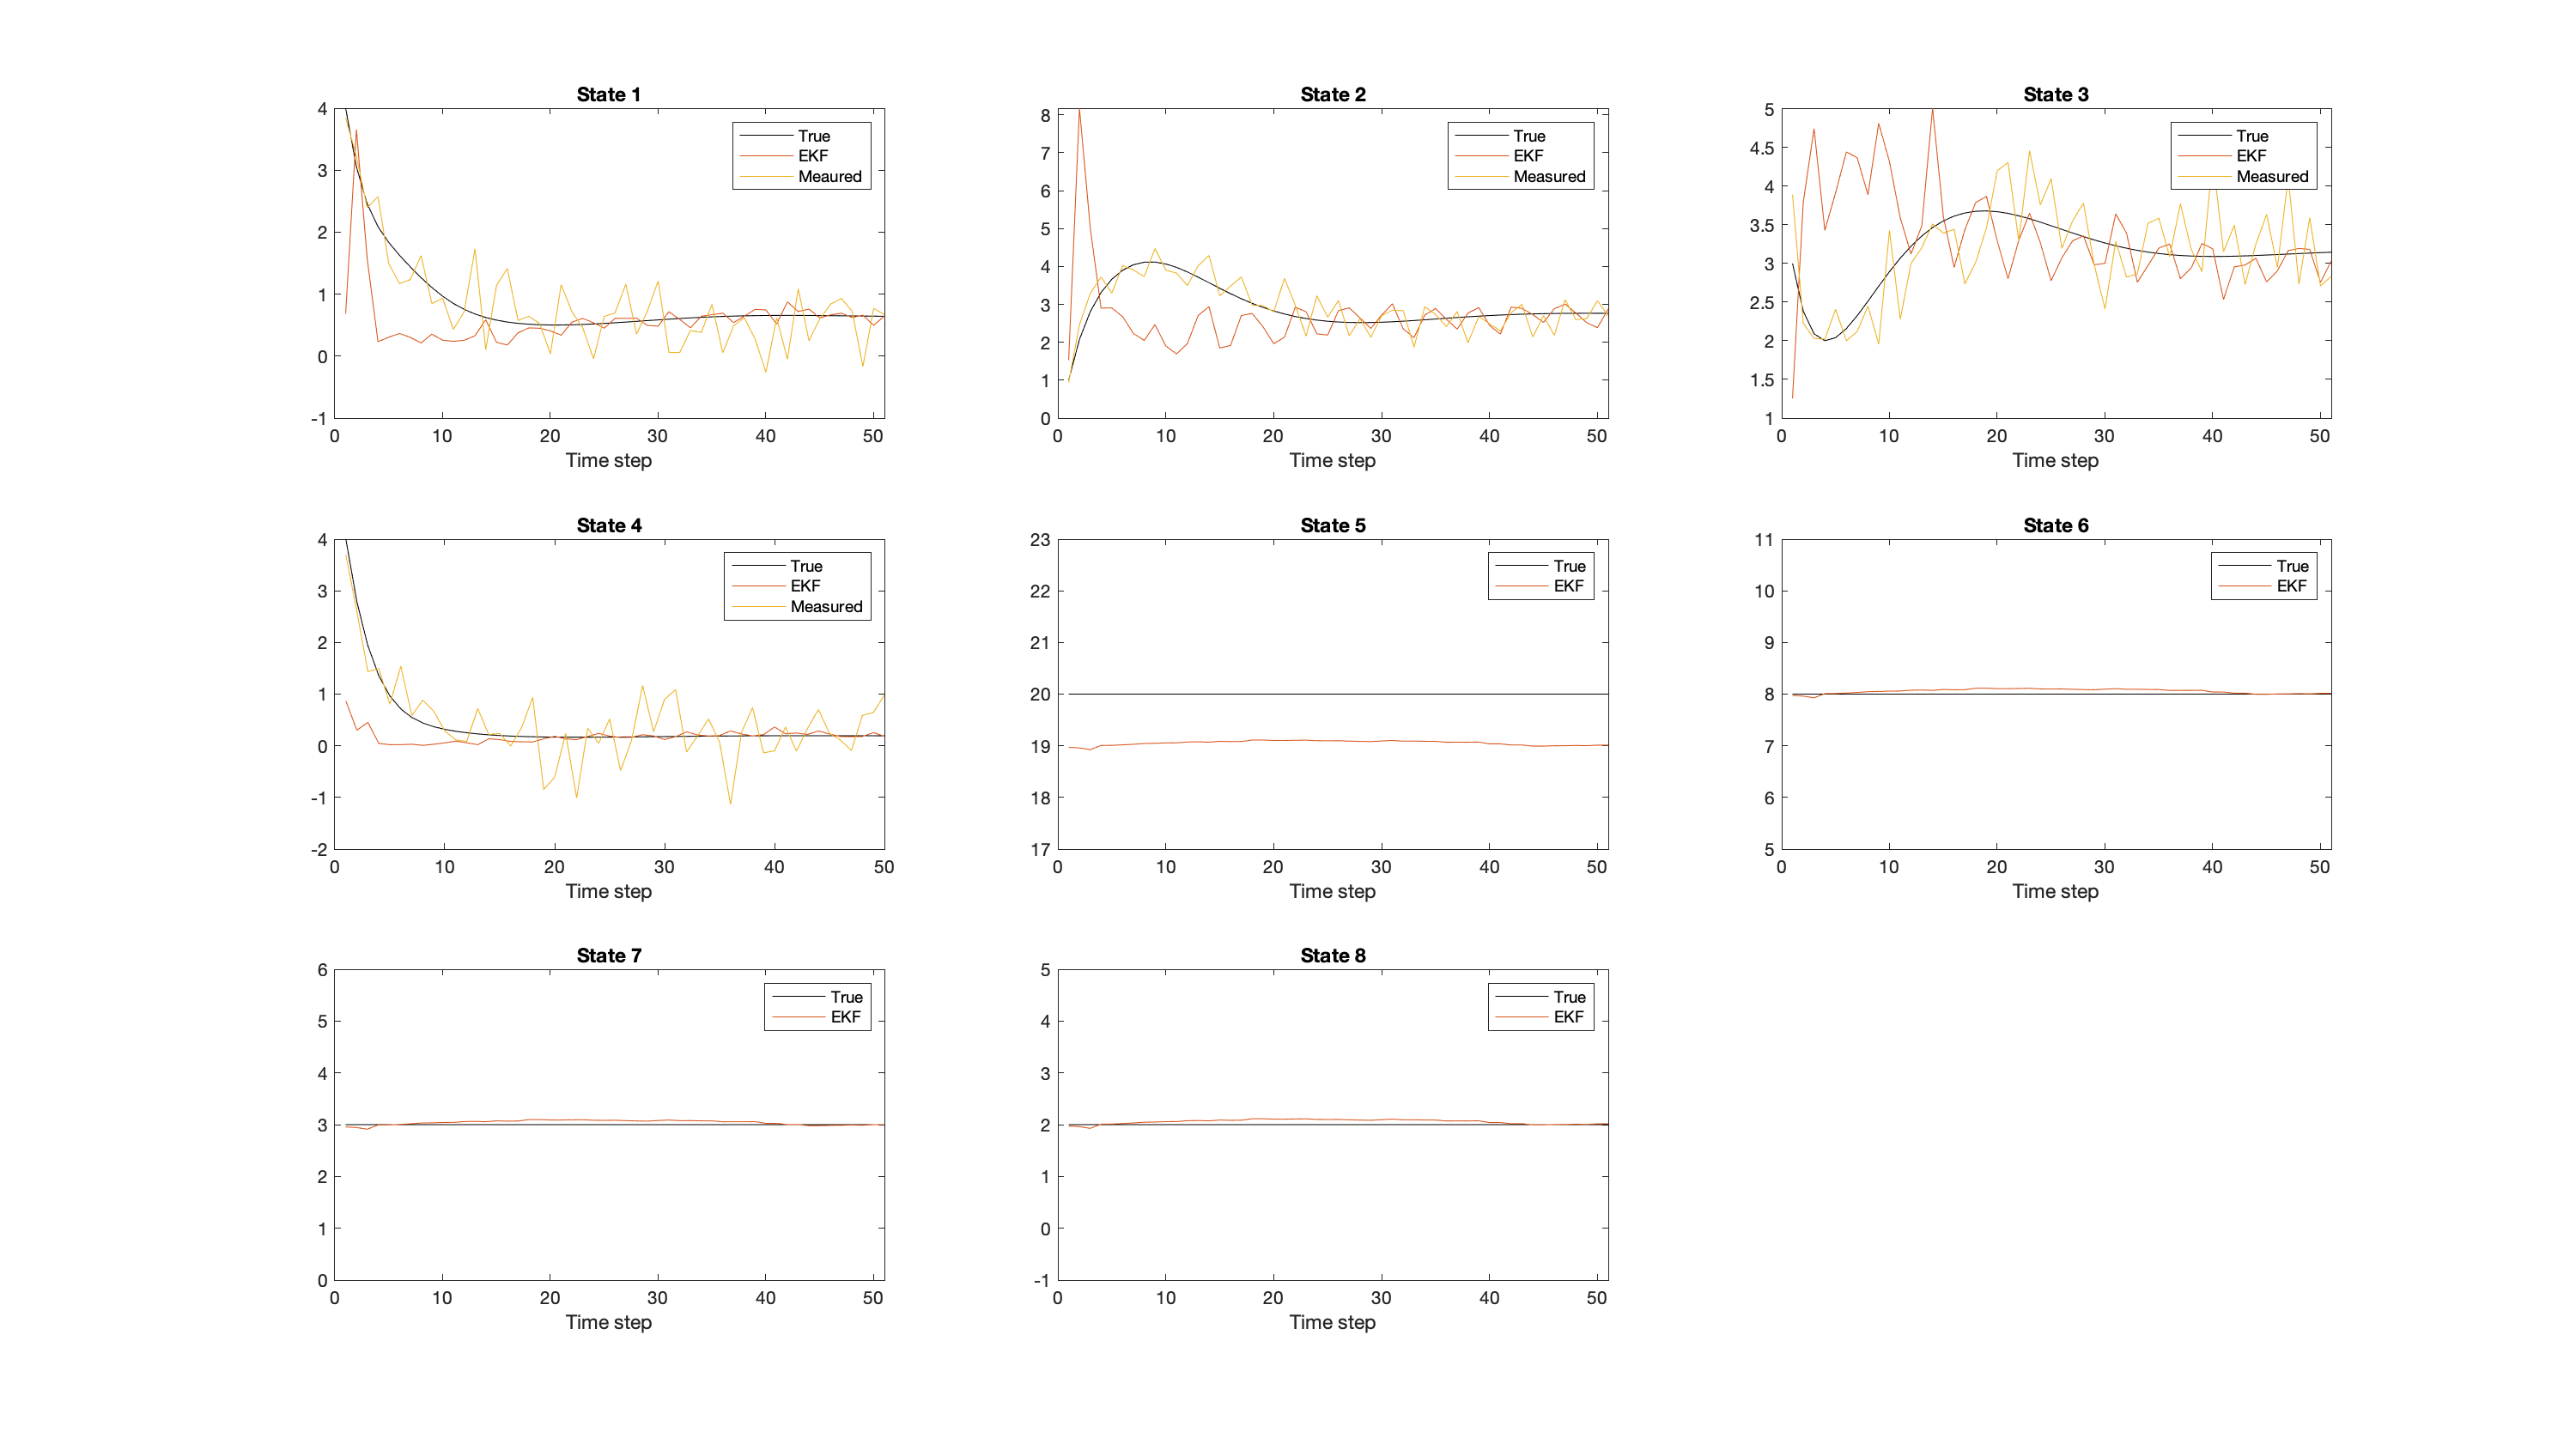
\includegraphics[scale = 0.6]{EKF_param_est.png}
    \caption{sdaasads}
\end{figure}


\noindent Residuals, also known as the innovation, are one way to access the model's performance. Recall that the residual is the difference between the actual measurement values and the predicted measurement values. Since only one state, $x1$ had incoming measurements, the residual graph in Figure 4.10 is specifically for $x1$. Generally, a strong residual graph has

\begin{itemize}
\item a symmetrical distribution that is clustered toward the center,
\item values that are close to 0,
\item a random or unclear pattern.
\end{itemize}


\textcolor{red}{ADD RESIDUAL GRAPH HERE}
\begin{figure}[h]
    \centering
    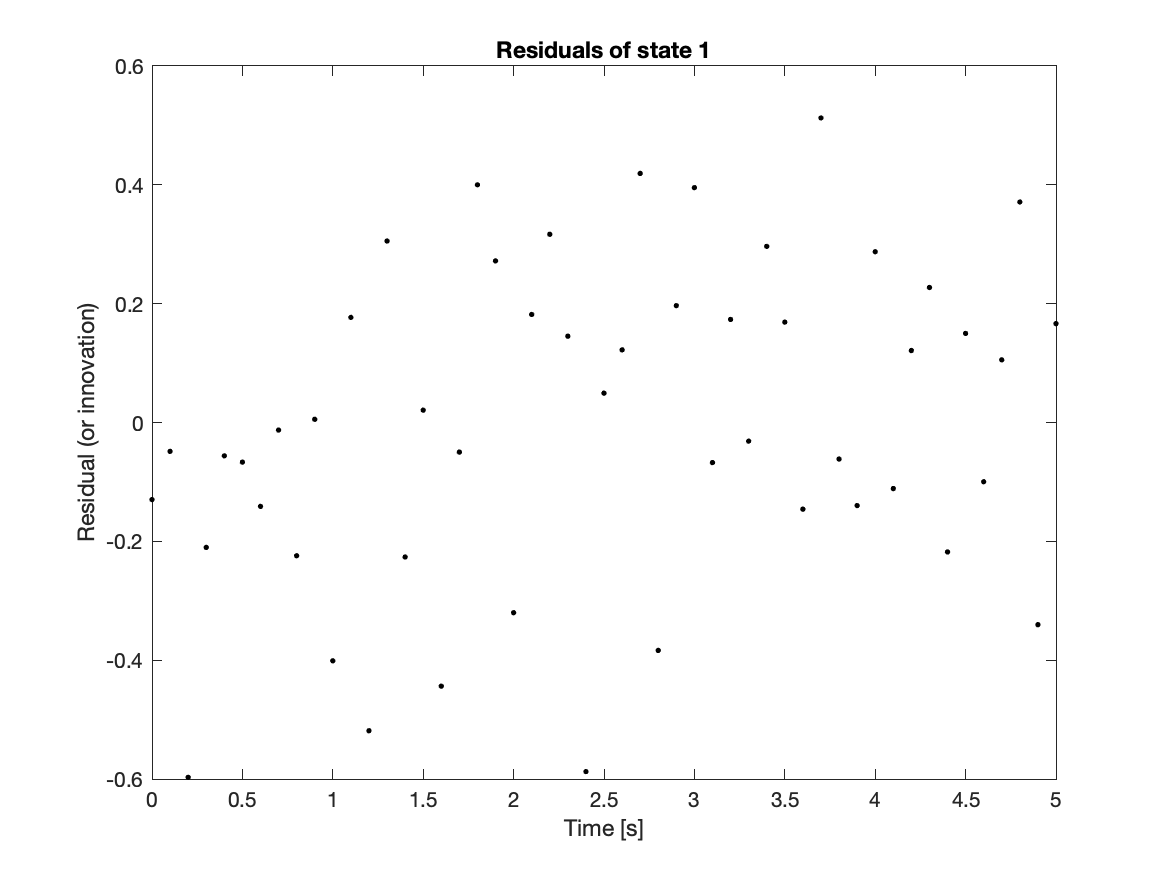
\includegraphics[scale = 0.6]{Meskin_residuals_state1.png}
    \caption{This scatterplot provides information regarding the residual, or innovation, of the first state, which is the only state recieving incoming system measurements.}
\end{figure}
















\chapter{Unscented Kalman Filters}
\label{Unscented Kalman Filters}

The Unscented Kalman Filter (UKF) is another nonlinear version of the Kalman Filter and was developed to address the shortcomings of the EKF. As opposed to using the Jacobian to linearly approximate around a single point, the UKF uses the Unscented Transform (UT) to approximate around multiple points, known as sigma points. The UT is a method of approximating probability distributions that have undergone a non linear transformation using limited statistics. The UT uses these sigma points, which are represented in a Sigma Point Matrix, to represent the normal distribution of the data. Then, the sigma points undergo a non-linear transformation, resulting in a posterior distribution that is not normal \cite{inbook, Wan01theunscented}. It is possible to approximate the normal distribution of the posterior distribution using the weights and covariance that were calculated prior to the transformation. A high level overview of this process is illustrated in Figure ~\ref{fig:UKF}. This process enables the Kalman Filter to be applied to more complex non linear problems. 

\begin{figure}[ht]
    \centering
    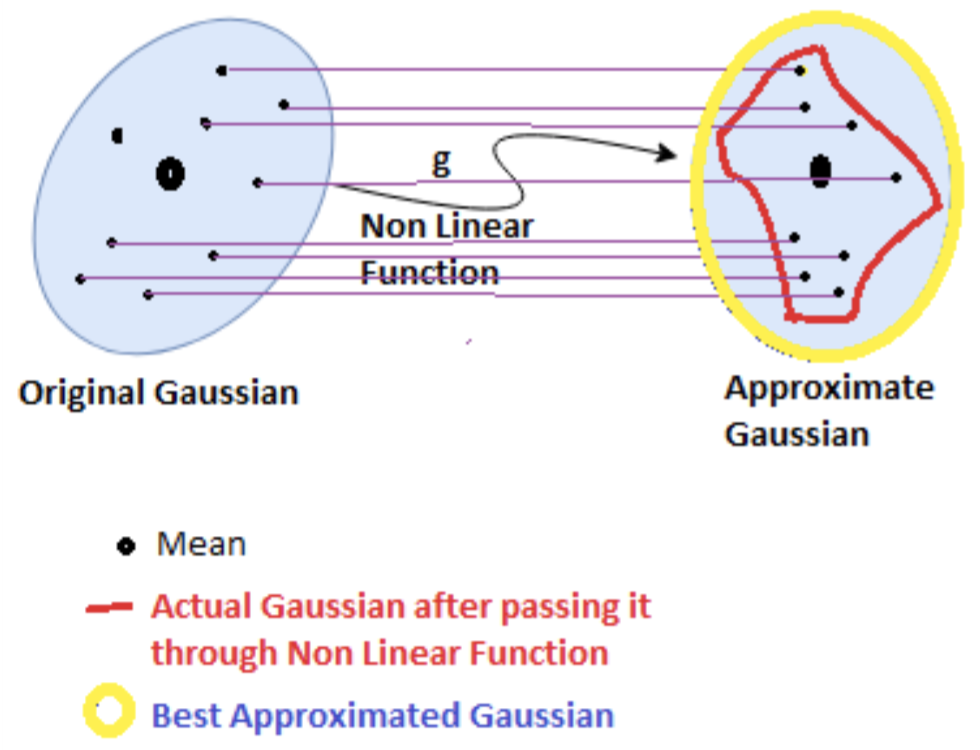
\includegraphics[scale = 0.35]{UKF.png}
    \caption{A depiction of the general overview of the UKF from \cite{chadha_2019}. Here we see that sigma points are sampled from a Gaussian distribution and are propagated through a non-linear function, called $g$. Though the output is non-Gaussian, an approximation of the Gaussian distribution can be obtained.}
    \label{fig:UKF}
\end{figure}


\newpage

\noindent Unlike the Kalman Filter and the Extended Kalman Filter, the UKF also has a set of parameters. Explanations of each parameter and their default values can be found in Table 4.2. Here, parameters are necessary for controlling the spread of sigma points. This was not needed for the EKF, since the EKF was only linearizing around the mean. The thesis will not be exploring how to tune these parameters, but one method to do so is through ad hoc testing.


\noindent The term 'unscented' was arbitrarily coined by the developer of the UKF, Jeffrey Uhlmann. In an interview, he shares:
\begin{displayquote}
"Initially I only referred to it as the “new filter.” Needing a more specific name, people in my lab began referring to it as the “Uhlmann filter,” which obviously isn’t a name that I could use, so I had to come up with an official term. One evening everyone else in the lab was at the Royal Opera House, and as I was working I noticed someone’s deodorant on a desk. The word “unscented” caught my eye as the perfect technical term. At first people in the lab thought it was absurd—which is okay because absurdity is my guiding principle—and that it wouldn’t catch on. My claim was that people simply accept technical terms as technical terms: for example, does anyone think about why a tree is called a tree?"
\end{displayquote}


\newpage

\section{Unscented Kalman Filter Algorithm}

\noindent Before delving into the details of the algorithm, we will explore a high-level overview of the UKF process. As with the KF and the EKF, the UKF follows the three major components of:
\begin{enumerate}
  \item Initializing the model's states
  \item Generating a prediction
  \item Updating prediction with measurements from the system.
\end{enumerate}

\noindent In the first step, initializing the model requires calculation of sigma points. These sigma points characterize the normal distribution of the data. 
\begin{figure}[h]
    \centering
    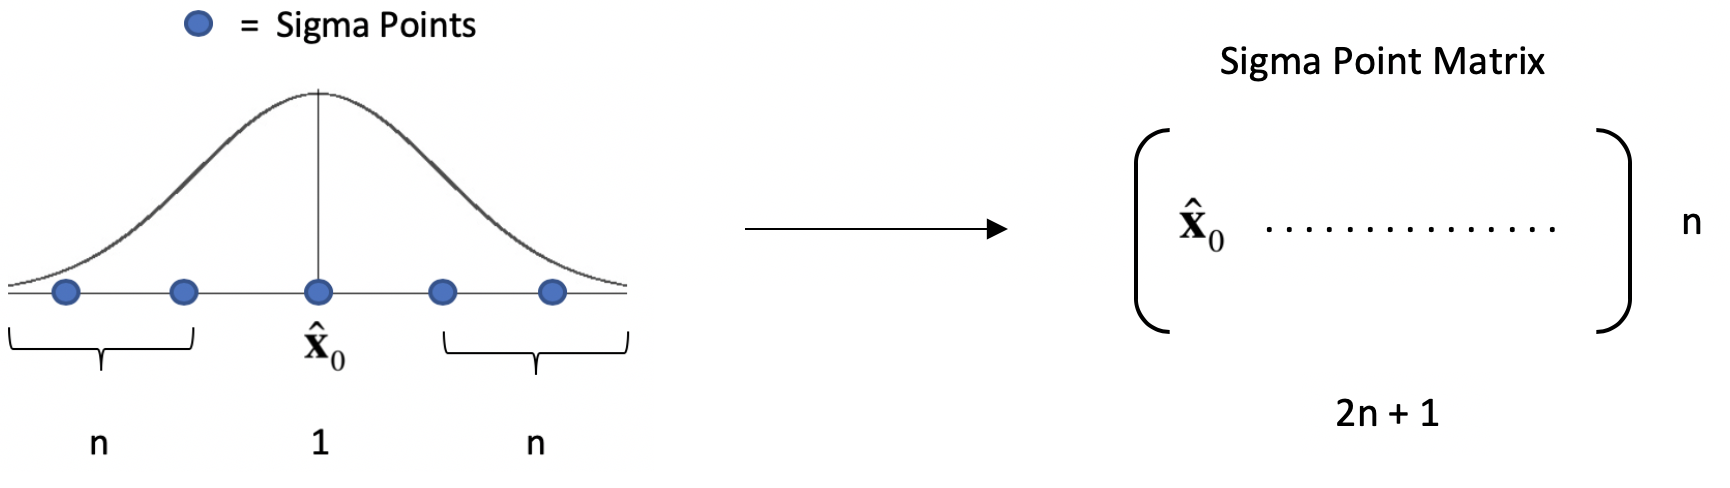
\includegraphics[scale = 0.4]{SPM.png}
    \caption{A brief illustration on how sigma points are used to characterize the Gaussian distribution of the data and how these sigma points are used to generate the Sigma Point Matrix.}
\end{figure}

\noindent After the sigma points undergo a nonlinear transformation, the resulting transformed sigma point matrix can be used to approximate the normal distribution of the data, which we can use to generate a prediction.
\begin{figure}[h]
    \centering
    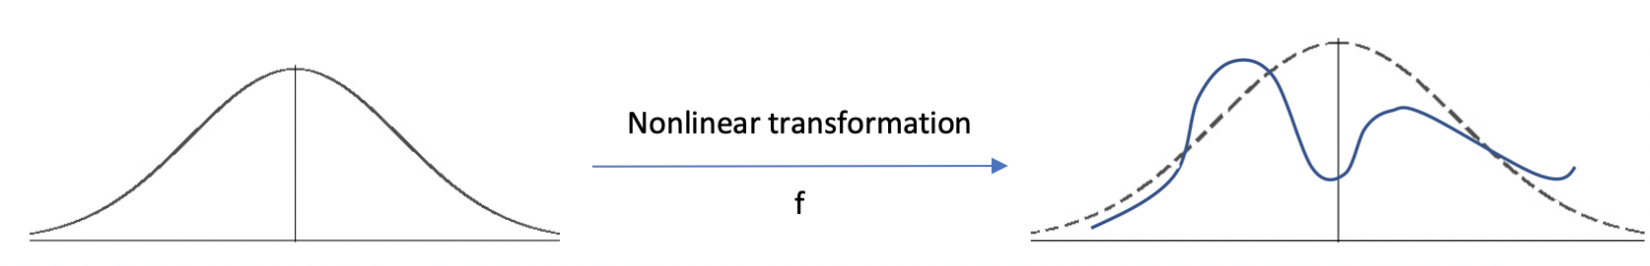
\includegraphics[scale = 0.45]{transform.png}
    \caption{After the Gaussian-distributed data undergoes a nonlinear transformation, call it $f$, the result is no longer linear}
\end{figure}

\newpage
\noindent One can see that this follows the basic outline of the previous versions of the KF, but the process of doing each step varies. More details about each step are explained below.

\begin{enumerate}
    \item The first step is to initialize state vector, $x_0$, and covariance, $P_{x_0}$, which is exactly similar to both the KF and the EKF. Since we know that the $x_0$ is normally distributed, the expectation can be calculated by
    \begin{align*}
    	x_0 = \mathbb{E}[x_0]   = \sum^n_{i = a} x_i p_i = [x_a p_a + x_b p_b + \hdots + x_n p_n]^T,
        %\hat{x}_{0} &= \mathbb{E}[x_{0}] 
    \end{align*}
   where $x_0= [x_a, x_b, \hdots, x_n]^T$, $p_a, p_b, \hdots, p_n$  is the respective probability of obtaining each state variable and $T$ is the transpose. Next initialize the state covariance, by
    \begin{align*}
        P_{x_{0}} &= \mathbb{E}[(x_{0}-\hat{x}_{0})(x_{0}-\hat{x}_{0})^{T}].
    \end{align*}
    
\noindent Unlike the KF and EKF, the UKF requires the calculation of sigma points, which is a way characterizing the distribution of the data. The number of sigma points is deterministic and depends on the dimensions of the system. In general, a UFK will have  $2x$ + 1 sigma points, where $x$ represents the dimension of the state vector \cite{inbook, inproceedings, Wan01theunscented}.  All sigma points are stored in a sigma point matrix, called $\chi$. To get a general idea about the distribution of the data, we use $\lambda$, which is a scalar value that determines how spread out the sigma points are from the mean. $\lambda$ can be calculated by
         \begin{align*}
        \lambda = \alpha^{2}(\text{x}+\kappa)-x,
         \end{align*}
         where x is a scalar representing the number of states in the system, and $\alpha$ and $\kappa$ are both parameters that control for the spread of sigma points around the mean value of the state. The spread of the sigma points is proportional to $\alpha$. For both $\alpha$ and $\kappa $,  the smaller the values are, the closer the sigma points are to the mean.\\ \\
       Another parameter of the UKF is $\beta$, which uses information regarding state distribution to adjust sigma points. $\beta$ has a default value of 2 if the data is Gaussian (which is an assumption we will make throughout this paper).  \\ \\
       Since the goal of this step is to characterize the distribution, set one of these sigma points to the mean, $\chi_{\ 0,k-1}$ which can be expressed as 
    \begin{align*}
        \chi_{\ 0,k-1} &= x_{k-1|k-1} ,
     \end{align*}
     where 0 is a row on $\chi$ and $k-1$ is the time step. Then allocate half of the remaining points will be smaller than the mean and the other half will be larger than the mean by
         \begin{align*}
        \chi_{\ i,k-1} &= x_{k-1|k-1} +  \bigg(\sqrt{(x+\lambda )P_{x,{k-1}}}\bigg)_{i} \quad \quad \quad i=1,\dots, x, 
        \end{align*}
         \begin{align*}
        \chi_{\ i,k-1} &= x_{k-1|k-1} - \bigg(\sqrt{(x+\lambda )P_{x_{k-1}}}\bigg)_{i-n} \quad \quad \quad i=x + 1,\dots,2x + 1,
        \end{align*}
        where x is the dimension of the state vector, $(\sqrt{(d_{x}+\lambda)P_{x_{k-1}}})$ is a matrix, and the $i$ subscript is the $i^{th}$ column of the matrix. 
        Recall that the square root of a matrix, satisfies the following condition: $A = B^2$, where $A$ and $B$ are both matrices. 
        
        
\noindent Next, we must calculate a weight for each sigma point. Weights are scalars used to calculate posterior sigma points after they have undergone a nonlinear transformation. One set of weights,  $W^{(m)}$, will be used to calculate the posterior mean while another set of weights $W^{(c)}$ will be used to calculate the posterior covariance. Weights can have positive or negative values, but will ultimately sum to 1 \cite{article6}. \\
        
\noindent The initialized weight for the mean, $W^{(m)}_{0} $ can be found by
            \begin{align*}
        W^{(m)}_{0} = \frac{\lambda}{x+ \lambda},
         \end{align*}
         where x is the number of states in the system. Similarly, the weight for the covariance at the initial time step, $W^{(c)}_{0}$, is given by
        \begin{align*}
        W^{(c)}_{0} = \frac{\lambda}{x+ \lambda} + (1 - \alpha^{2} + \beta).
         \end{align*}
          In later time steps, $W^{(m)}_{i} $ and $W^{(c)}_{i}$ follow the same equation, given by
               \begin{align*}
        W^{(m)}_{i} = W^{(c)}_{i} = \frac{\lambda}{2(x + \lambda) } \quad \quad \quad i=1,\dots,2x.
            \end{align*}
           
          
           
        \item A prediction can be generated by performing a nonlinear transformation on the sigma point matrix, $\chi$, in order to generate a prediction and provide an update on the covariance matrix. After $\chi$ undergoes a nonlinear transformation, $f$, the result is a transformed sigma point matrix at time step $k$ given the last time step, $k-1$, which will is called $\chi_{k | k - 1}$ and is given by
        \begin{align*}
        \chi_{k | k - 1} = f(\chi).
        \end{align*}
        
        
        Though $\chi$ has a Gaussian distribution,  $ \chi_{k | k - 1} $ does not because it has been transformed by the nonlinear state function $f$. The sum of the columns in $ \chi_{k | k - 1} $ and the weights calculated in step 3 will then be used to generate a prediction of the state variables, $x_k$, by 
        \begin{align*}
         x_{k|k-1} = \sum^{2x}_{i = 0} W_i^{(m)} \chi_{i, k | k - 1}.
        \end{align*}
       Adding the weights help approximate the Gaussian distribution of the state variables after they undergo a transformation. 
       
        
                \item Now that the prediction component of the filter is completed, we move on to the correction step, which begins by calculting the transformed covariance matrix and then transforming our predictions into a format that can be compared with system measurements. Calculation of the posterior (also called augmented) sigma points is necessary for converting system measurements into a format that can be compared with the state variables. System measurements must undergo a non linear transformation, $h$, resulting in a non Gaussian distribution. Therefore, the Unscented Transform is used again.
                Begin by calculating the posterior covariance matrix for the state variable, which is necessary for updating the state covariance later on by
        \begin{align*}
        P_{x, k | k-1} = \sum^{2x}_{i = 0} W_i^{(c)} (\chi_{i, k | k - 1} -   x_{k|k-1} )(\chi_{i, k | k - 1} - x_{k|k-1} )^T + Q,
        \end{align*} 
        where $Q$ is process noise that provides the error in our model $f$, $T$ is the transpose, and $W_i^{(c)}$ are the weights calculated earlier. \\     
                
\noindent Then calculate augmented sigma points, $\chi^{(aug)}$, by
      \begin{align*}
        \chi^{(aug)}_{0, k|k-1} =  x_{k|k-1}
        \end{align*}
         \begin{align*}
        \chi^{(aug)}_{ i,k |k-1} &= x_{k|k-1}  \pm \bigg(\sqrt{(x+\lambda)P_{x_k}} \bigg)_{i} \quad \quad \quad  i=1,\dots,2x
        \end{align*}
        Recall that $\lambda$ was calculated in step 2. Since $\lambda$ is not time dependent, we can use the same value used earlier. \\ \\
        Now we calculate a sigma point matrix that represents the transformation of the prediction so that it can be compared with the states. This is necessary, especially in cases where measurements are not being obtained for all state variables. This sigma point matrix, $\mathcal{Y}_{k|k-1}$, can be obtained by having the $\chi_{k|k-1}$ undergo nonlinear transformation $h$, by
         \begin{align*}
       \mathcal{Y}_{k|k-1} = h(\chi^{(aug)}_{k|k-1}).
       \end{align*}
       $\mathcal{Y}_{k|k-1} $ is a transformed sigma point matrix. While in this format, it cannot be compared with the state variables. However, $\mathcal{Y}_{k|k-1}$ can be used to convert the system measurements into a format, $y_{k} $, which can be found by 
       \begin{align*}
       y_{k} = \sum^{2x}_{i = 0} W_i^{(m)}  \mathcal{Y}_{i, k | k - 1}.
       \end{align*}
       Now, the prediction can be compared with actual system measurements.
       
              
       Then, we are able to calculate the Kalman Gain in order to determine how much to correct the model. \\ \\
       Unlike previous versions of the KF, in addition to calculating the covariance of the state variables, calculations is also done for the covariance of observations, $P_{y}$, and for state variables with observations, $P_{xy}$. When generating the covariance matrix for $P_{y}$ the covariance of measurement noise is added. $P_{y}$ can be found by
        \begin{align*}
       P_{y, k | k-1} = \sum^{2x}_{i = 0} W_i^{(c)} (\mathcal{Y}_{i, k | k - 1} -   y_{k} )(\mathcal{Y}_{i, k | k - 1} -  y_{k} )^T + R,
       \end{align*}
       where $R$ is the covariance of measurement noise and $W_i^{(c)} $ are the weights calculated in step 3. Next, calculate $P_{xy}$ by
        \begin{align*}
       P_{xy, k | k-1} = \sum^{2x}_{i = 0} W_i^{(c)} (\chi^{(aug)}_{i, k | k - 1} -   x_{k } )(\mathcal{Y}_{i, k | k - 1} -  y_{ k } )^T .
       \end{align*}
       Finally, using $P_{y}$ and $P_{xy}$, calculate the Kalman Gain, by
       \begin{align*}
       K_k = P_{xy, k | k-1} (P_{y, k | k-1}) ^{-1}.
       \end{align*}
        
        
        
      \noindent Finally, we are able to correct the prediction and updating the covariance matrix, which will both be used in the next iteration. Similar to the UKF and the KF, the prediction of the state variables at the next time step, $x_{k+1}$, is given by 
      \begin{align*}
        x_{k|k} = x_{k|k-1} + K_k(\hat y_k - y_{k}),
        \end{align*}
        where $\hat{y}_k$ is system measurements. Conclude this iteration of the filter by preparing $ P_{x, k} $ for the next iteration.  $P_{x, k} $ can be found by
       \begin{align*}
       P_{x, k|k} = P_{x, k|k-1} -K_k (P_{y, k | k-1} ) {K_k}^T.
       \end{align*}     
  
  \end{enumerate}          
    
\newpage        

\noindent In conclusion, the UKF is a nonlinear version of the KF that addresses the shortcomings of the EKF. Unlike the EKF, the UKF linearizes around multiple points, which results in a better approximation of the nonlinear system. The algorithm for the UKF involves calculating sigma points, which are values that characterize the Gaussian distribution of the system, and weights. Using these weights and sigma points, it is possible to approximate the Gaussian distribution of a system after it undergoes a nonlinear transformation. This process is known as the Unscented Transform. In addition, this model can be tuned to adjust the spread of sigma points using the $\alpha, \beta, $ and $\kappa$ hyper-parameters. A summary of all of the parameters and hyper-parameters used in the UKF can be found in Table ~\ref{tab:UKF} and Table ~\ref{tab:hyperparam} respectively. 

    
\begin{center}
\begin{table}[h]
\centering
\caption{Description of all variables in the Unscented Kalman Filter} \label{tab:sometab}
\begin{tabular}{ |p{2cm}||p{5cm}|p{2cm}| }
    \hline
    \multicolumn{3}{|c|}{Variables in the Unscented Kalman Filter } \\ 
    \hline
    Variable & Description & Dimensions \\
    \hline
    $x$ & State variables & $ x \times 1 $\\ 
    $y$ & Transformed prediction & $y \times 1 $\\ 
    $\hat y$ & Sytem measurements & $y \times 1 $\\ 
    $\chi $ & Sigma point matrix for states&$ x \times (2x + 1) $\\
    $\mathcal{Y}$ & Sigma point matrix for obs &$ y \times (2x + 1) $\\
    $f$ & Nonlinear state function & $x \times 1 $  \\ 
    $h$ & Nonlinear observation function & $y \times 1$\\
    $P_x$ & Covariance of states & $x \times x $  \\
    $P_y$ & Covariance of observations& $y \times y $  \\
    $P_{xy}$ & Covariance of states/obs& $x \times y $  \\
    $Q$ & Process noise covariance & $x \times x $  \\
    $R$ & Measurement noise covariance & $y \times y $  \\
    $W^{(m)}$ & Weight for posterior mean & scalar \\
    $W^{(c)}$ & Weight for posterior covariance & scalar \\
    \hline
\end{tabular} 

\end{table}
\label{tab:UKF}
\end{center}


\begin{center}
\begin{table}[h]
\centering
\caption{Description of all hyper-parameters in the Unscented Kalman Filter} \label{tab:sometab}
\begin{tabular}{ |p{1cm}||p{5cm}|p{2cm}| p{1cm}| }
    \hline
    \multicolumn{4}{|c|}{Hyper-Parameters in the Unscented Kalman Filter } \\ 
    \hline
     & Description & Bounds & Default \\
    \hline
    $\alpha$ & Controls spread of sigma points & $0 < \alpha \leq 1$ & $.001$\\
    $\beta$ & Adjust sigma point weight & $\beta \geq 0$ & 2\\
    $\kappa $ & Sigma point weighting constant & $0 \leq \kappa \leq 3 $  & 0 \\
    \hline
\end{tabular}
\end{table}
\label{tab:hyperparam}
\end{center}
            
            
            
            
            
            
    
  
\section{Van der Pol Example}
\label{Van der Pol Example}


Applying the UKF to the Van der Pol oscillator will be used as a simple example to demonstrate the impacts of measurement and process noise. The Van der Pol equation, so named after its developer Balthasar Van der Pol, describes a self sustaining oscillator that create energy at small amplitudes and remove energy from large amplitudes. The Van der Pol equation describes a nonconservative oscillator (also known as a relaxation oscillator). Applications of the Van der Pol oscillators include circuits, vacuums, and modeling biological systems
 \cite{weisstein_2019}. The Van der Pol oscillator is represented by a nonlinear second order differential equation: 
\begin{align*}
\frac{d^2y}{dt^2} + \mu(y^2-1)\frac{dy}{dt} = 0
\end{align*}   \\
where $\mu$ is a damping coefficient, $\frac{d^2y}{dt^2}$ is acceleration, $\frac{dy}{dt}$ is velocity, and $y$ is position. Therefore, for all $\mu < 0$, dampening occurs and the system tends to 0. The rate at which the system converges to zero is dependent on the size of $\mu$, with larger values taking longer to converge and smaller values converging faster. If $\mu = 0$, the system becomes a simple harmonic oscillator, where motion is periodic. Lastly, if $\mu > 0$, the system enters a limit cycle, which is an isolated closed trajectory. \cite{kinoshita_2013}. \\ 

\noindent The UKF can be applied to this nonlinear system to determine where the system will be at a point in time. To do so, relevant state variables include position and velocity.  \footnote{In Matlab, x(1) and x(2) represent position and velocity, respectively}
\begin{align*}
x_k = \begin{bmatrix}
          y\\ 
          v
           \end{bmatrix}  
\end{align*}


\noindent Transforming the Van der Pol equation from a second order differential equation to a first order differential equation makes it easier to define $f$, the state function of the system. By substituting $v$ for $\frac{dy}{dt}$, and $ \frac{dv}{dt} $ for  $\frac{d^2y}{dt^2}$ one can rewrite the Van der Pol equation as 
  \begin{align*}
 	\frac{dv}{dt}  +\mu(y ^2-1)v + y = 0.
 \end{align*}

\noindent From this, we get the differential equations associated with the state variables to generate the nonlinear transformation function $f$. For the sake of simplicity, assuming $\mu = 1$, we get
\begin{align*}
\dot x_k  = 
	\begin{bmatrix}
           \frac{dy}{dt}  \\ \\
           \frac{d^2y}{dt^2} 
           \end{bmatrix} = 
           \begin{bmatrix}
          v \\ \\
           \frac{dv}{dt} 
           \end{bmatrix}  =
           \begin{bmatrix}
           v \\ \\
           -1 (y^2 - 1)v - y 
           \end{bmatrix}=
           \begin{bmatrix}
           0 & 1 \\ \\
           -1& 1- y^2 - 
           \end{bmatrix} x_k 
           =
           f.
\end{align*}


\noindent In this particular example, the only measurement received from the system is position. Therefore, this filter is continually correcting for the position state state variable through measurement function $h$. Here, measurements of the system are simulated by adding noise to the position state variable. Even though there are only measurements for one state variable, we can still generate estimates of both state variables. In terms of parameters $\alpha, \kappa$, and $\beta$, default values were used.\\ 

\noindent To simulate a Van der Pol Oscillator, an ordinary differential equation solver can be applied to state function $f$ to generate true values of the system. Of course, systems do not perform perfectly; variations in model performance can be captured by randomly adding noise to the system. \\

\noindent All of this can be modeled on Matlab; all source code is from Matlab and can be referenced in Appendix A \cite{matlab /& simulink}

\begin{figure}[h]
    \centering
    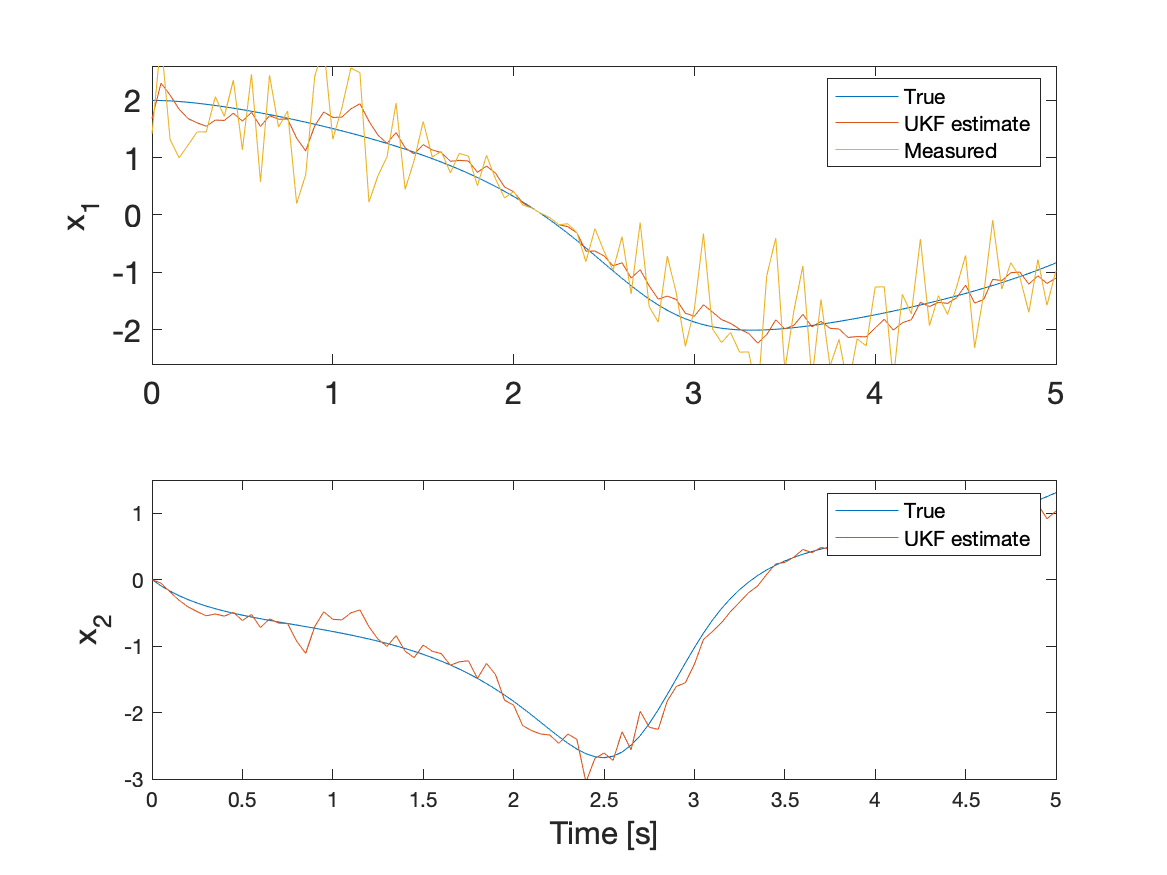
\includegraphics[scale = 0.6]{VDP.png}
    \caption{Performance of the UKF with R = 0.2, and Q = (0.02 0.1).
    As expected, the model converges on the true values of the system for both state variables. In this case, the only measurements we are receiving from the system are position, which is why the second state variable has no measured values.}
\end{figure}
\begin{figure}[h]
    \centering
    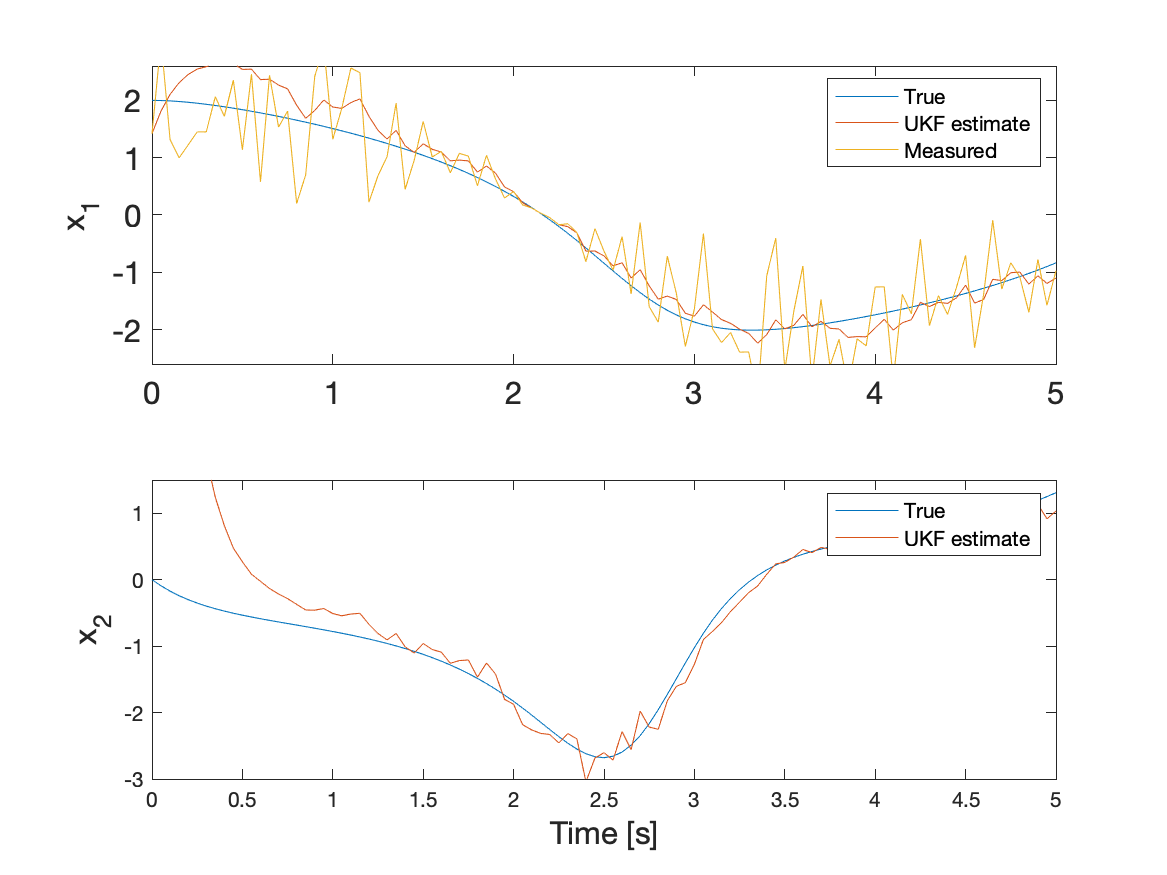
\includegraphics[scale = 0.6]{VDP_badinitial.png}
    \caption{Performance of the UKF with poor initial conditions: (1, 7)  instead of (2,0). Recall that inaccurate intial conditions cause convergence to take place more slowly. This seems to be the case, especially in the state variable that is not being corrected for.}
\end{figure}


\begin{figure}[!tbp]
  \centering
  \subfloat[UKF with high measurement noise (0.9)]{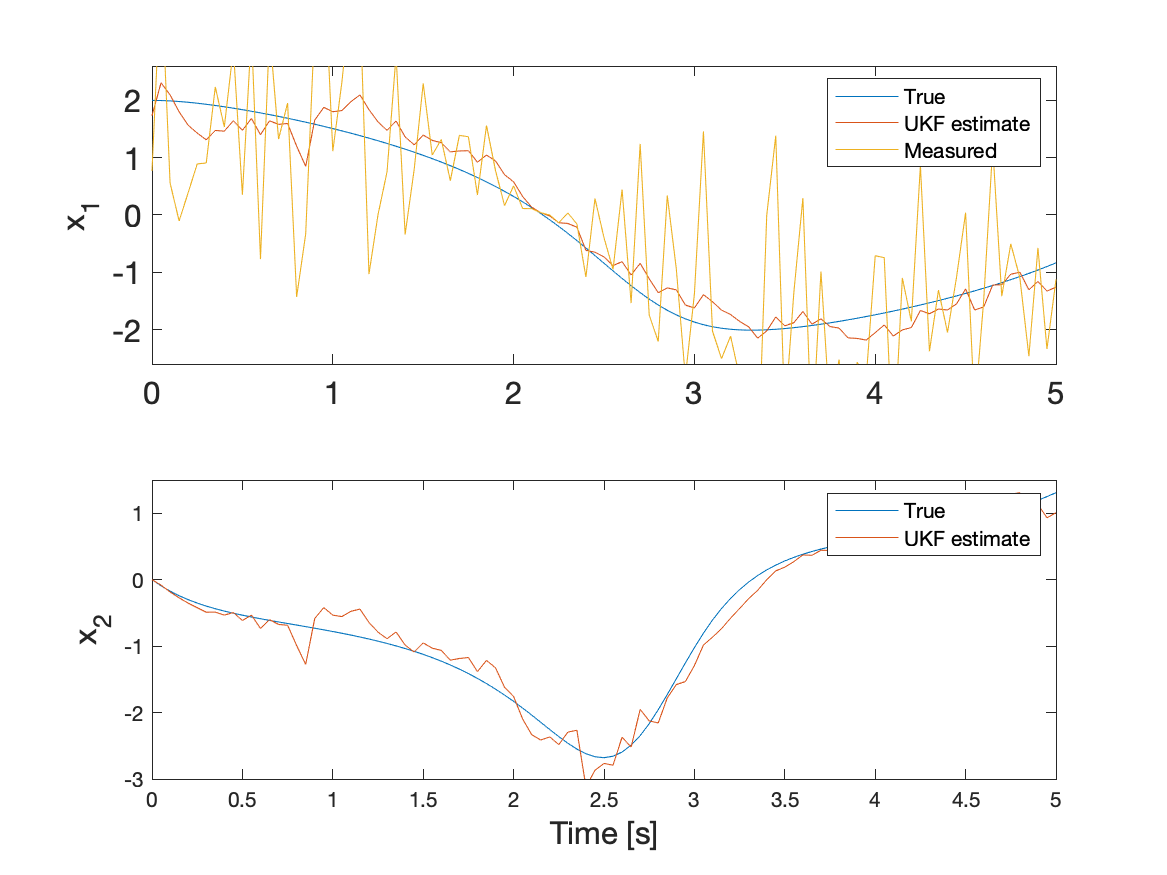
\includegraphics[width=0.5\textwidth]{VDP_highMN.png}\label{fig:f1}}
  \hfill
  \subfloat[UKF with low measurement noise (0.002)]{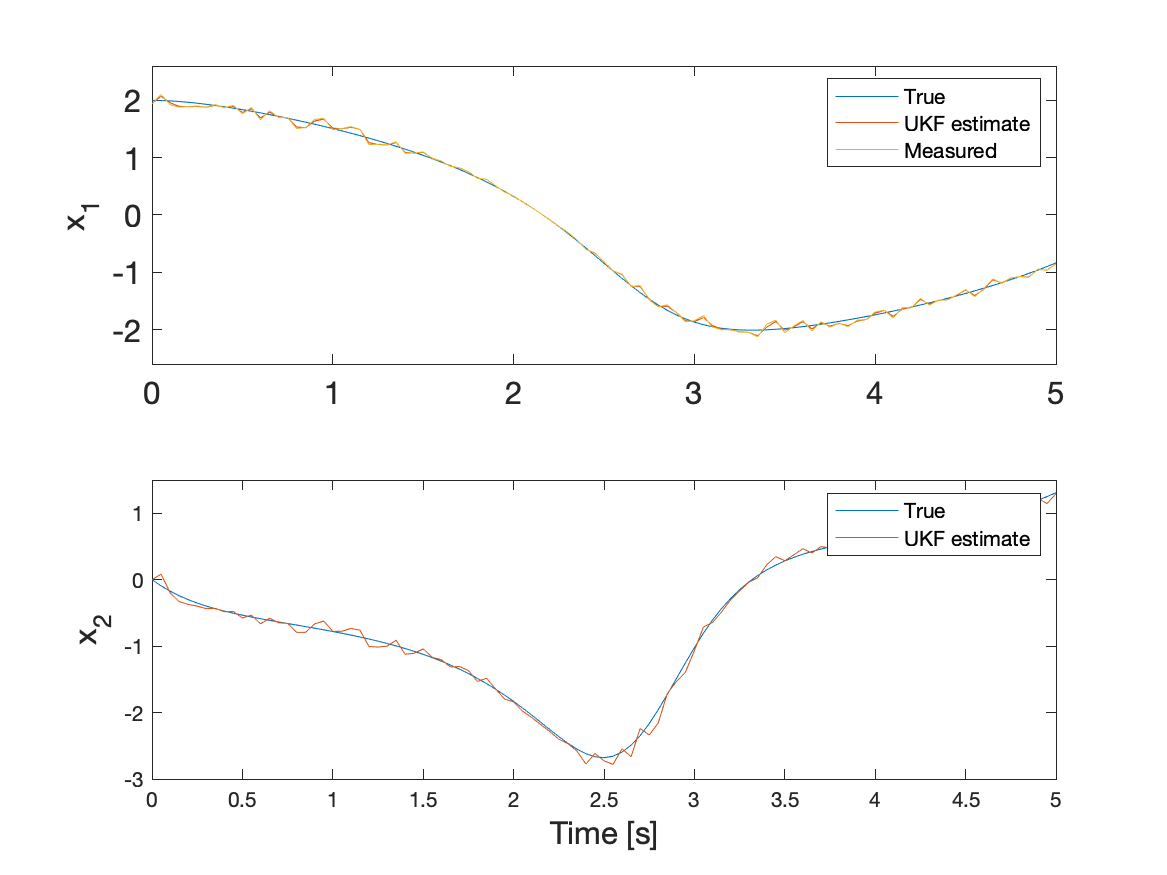
\includegraphics[width=0.5\textwidth]{VDP_lowMN.png}\label{fig:f2}}
  \caption{UKF on VDP oscillator with difference values of measurement noise.
  The model's behavior changes in response to the different values of measurement noise. Even when measurement noise is high, the UKF continues to perform well. Though, the rate of convergence appears to be slower.
On the other hand, when measurement noise is low, the UKF seems to converge instantly with the measured values. The velocity state variable also  quickly converges with the true value of the system.}
\end{figure}

\begin{figure}[!tbp]
  \centering
  \subfloat[UKF with high process noise (0.9 0.8)]{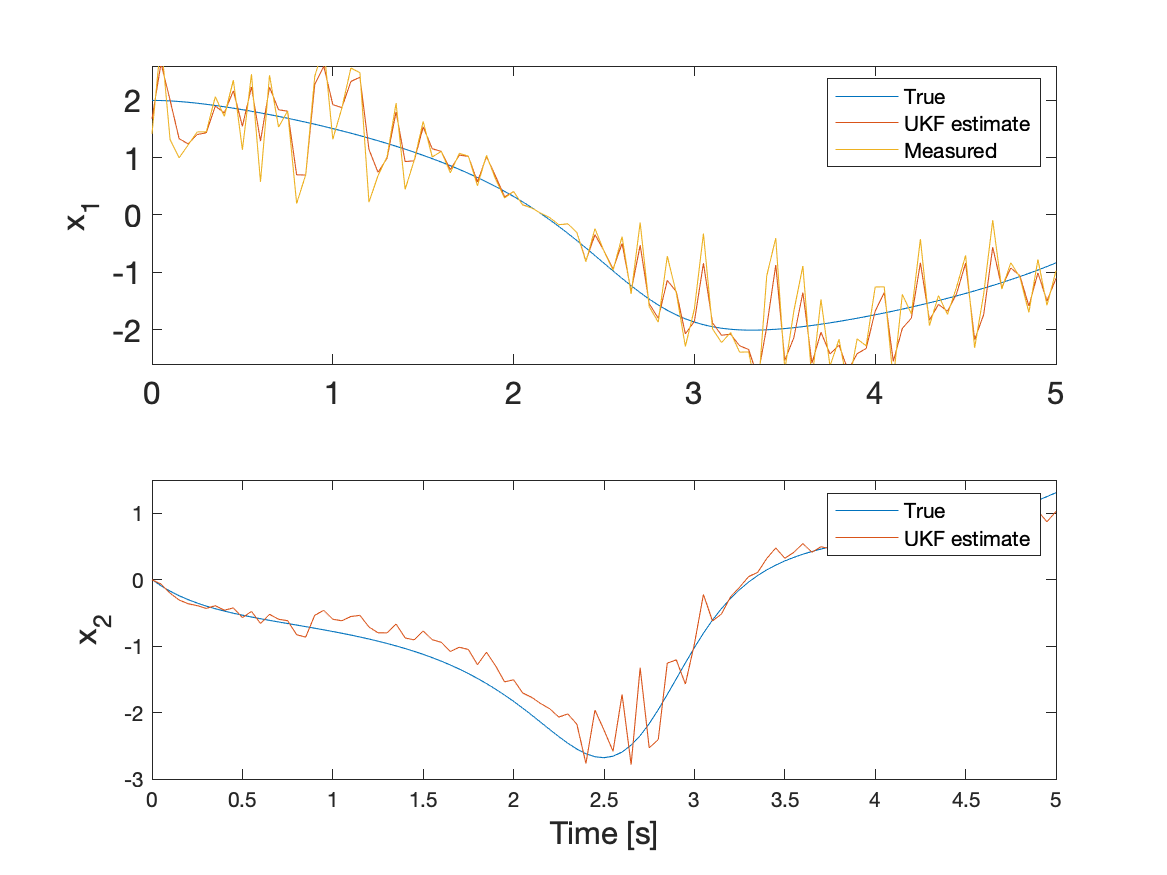
\includegraphics[width=0.5\textwidth]{VDP_highPN.png}\label{fig:f1}}
  \hfill
  \subfloat[UKF with low process noise (0.0001 0.0001)]{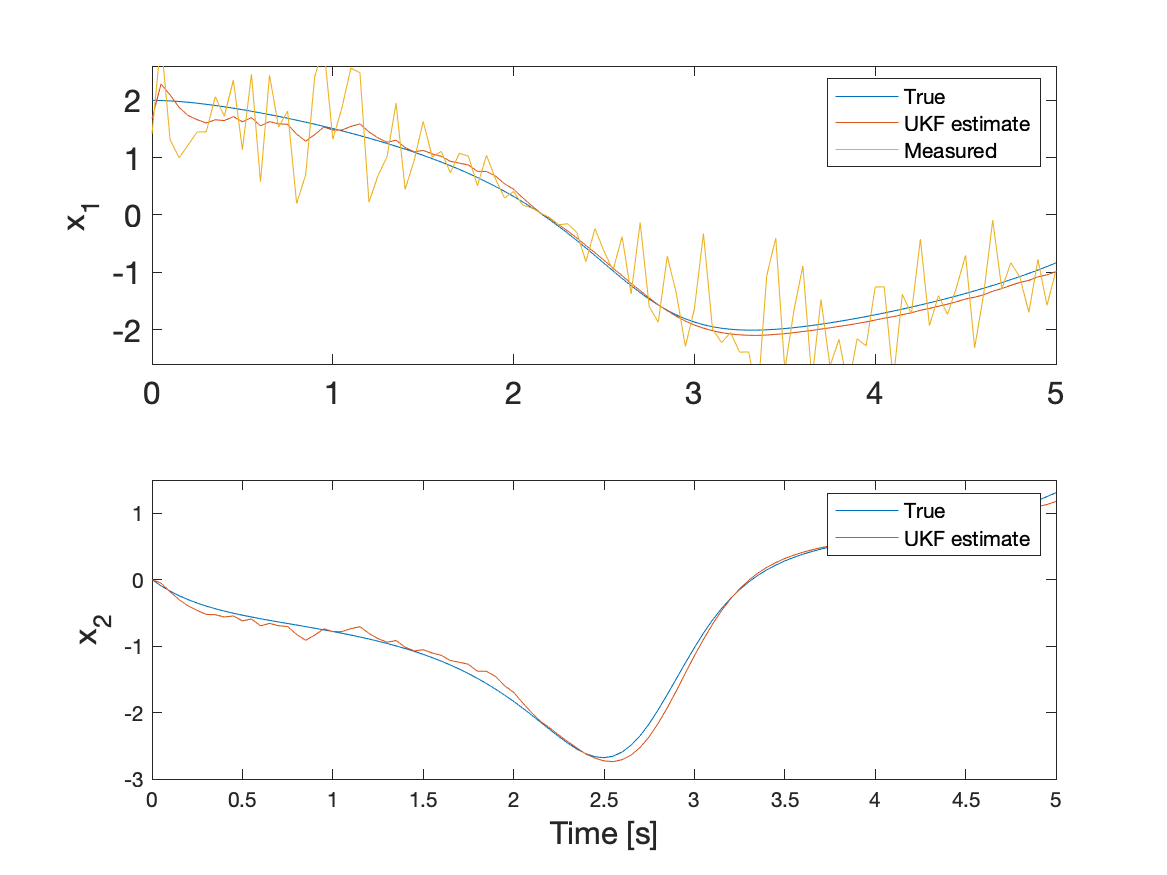
\includegraphics[width=0.5\textwidth]{VDP_lowPN.png}\label{fig:f2}}
  \caption{UKF on VDP oscillator with different values of process noise.
  Recall that process noise measures errors in the model. For the purpose of this example, process error was set to extreme high and low values. In theory, the Van der Pol equation should have small process error because it is a well used equation.}
   
\end{figure}
 

\section{Modeling Metabolites using UKF}
\label{Modeling Metabolites using UKF}




\noindent This is the same system explored in chapter~\ref{chap:EKF_Meskin}, but explored in the context of using an UKF as opposed to an EKF. The original research used an adaptation of the UKF, called the Iterative Unscented Kalman Filter (IUKF), to model the biological pathway of metabolites. Recall that this model contains four different states and 18 unknown parameters. These researchers utilized the IUKF for parameter fitting and was useful in enabling the model converge faster by resetting the covariance to re-excite the model. By not resetting the covariance at this step (as is done in the UKF), the three state variables without measurements converge significantly slower in this model. Utilizing the IUKF on this model was effective, because data regarding metabolites is highly influenced by noise, which is a factor that makes other approaches, such as regression and annealing, fail \cite{article5}. \\ 

\noindent In the paper, researchers had access to their own data sources and used an approach that was adapted from the UKF. Though we are not using their exact dataset, we will be simulating data using the same approach as the previous example. However, this example will be following UKF algorithm, as opposed to the IUKF algorithm. By doing so, the state variables without incoming measurements converge significantly slower than the measurable states. Ultimately, the goal of this example is to demonstrate how the UKF works on higher dimensional and more complex systems and how the UKF can be utilized in parameter estimation. \\

\noindent Recall that the four metabolites have the following differential equations:
\begin{align*}
\dot x_1 &= \alpha_1 x_3^{g_{13}} - \beta_1 x_1^{h_{11}}, \\
\dot x_2 &= \alpha_2 x_1^{g_{21}} - \beta_2 x_2^{h_{22}}, \\
\dot x_3 &= \alpha_3 x_2^{g_{32}} - \beta_3 x_3^{h_{33}} x_4^{h_{34}}, \\
\dot x_4 &= \alpha_4  x_1^{g_{41}} - \beta_4 x_4^{h_{44}},
\end{align*}
with 17 parameters ($\alpha_1, \hdots, \alpha_4, \beta_1, \hdots, \beta_4, g_{13}, g_{21}, g_{32}, g_{41}, h_{11}, h_{22}, h_{33}, h_{34},h_{44} $). In both the original example as well as this one, sampling time will be 0.1 seconds for 5 seconds, totaling 50 UKF estimates. Recall that data is simulated on MATLAB and the model is initialized with state variable $x_0 = [4, 1, 3, 4]^T$ and the state covariance to $P_0 = .01I$. \\

\noindent In the original example, researchers used the following hyper-parameter values: $\epsilon = 1, \kappa = -14$. In theory, values of $\kappa$ can be negative, but negative hyper-parameter values cannot be inputted into MATLAB. For this example, the hyper-parameter values used in this example are set to Matlab default values ($\alpha = 1e-3, \beta = 2, \kappa = 0$). The performance of the UKF on this system with these default hyper parameter values is shown in Figure ~\ref{fig:UKF_states}. Future work includes looking into ways to tune this hyper-parameters. \\

\comment{
\noindent Since the first state, $x1$ is the only state that has incoming system measurements, we have a 3 different blue lines in this figure. From this figure, it appears that the UKF prediction perfectly overlaps with the measured values. However, upon closer inspection, it actually does not. This is likely because there is only a small amount of measurement noise to the system. Figure 4.9 highlights the same information as Figure 4.8, but separates the states into different graphs, enabling a clearer illustration of each state's behavior.
}

\begin{figure}[ht]
    \centering
    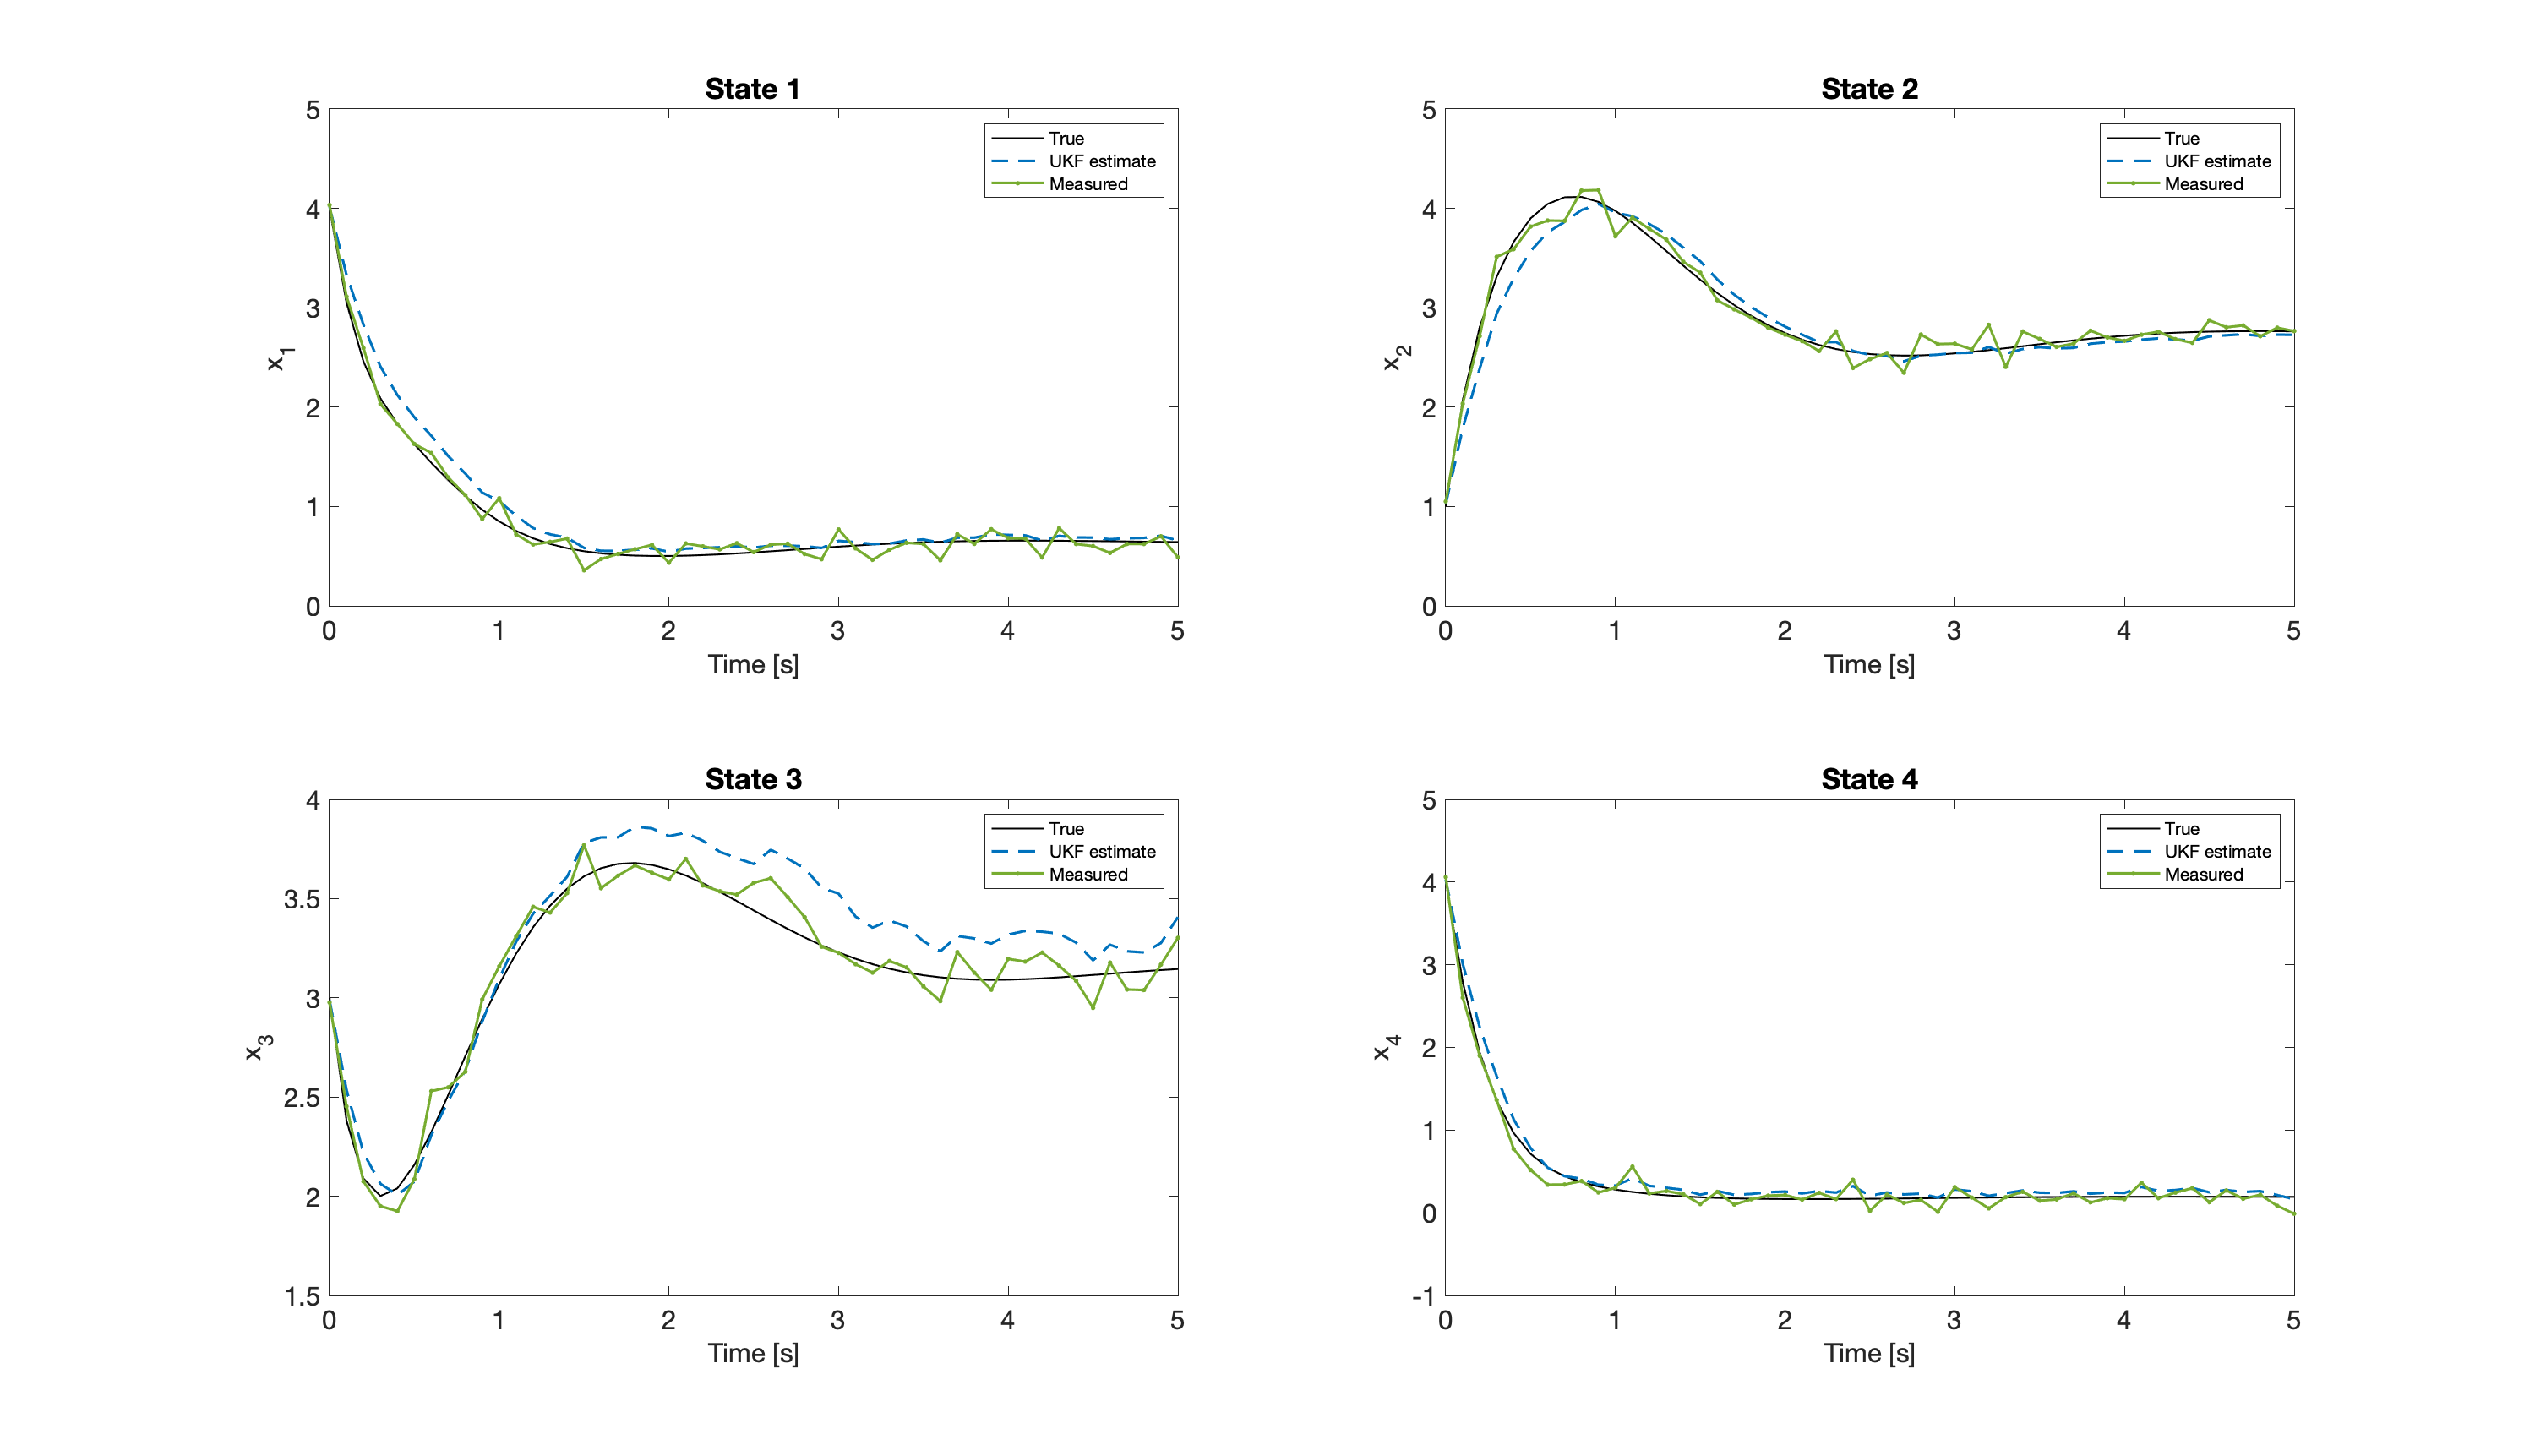
\includegraphics[scale = 0.3]{UKF_states.png}
    \caption{Performance of all four state variables with all four states being corrected. The model is initialized with $x_0 = [4, 1, 3, 4]^T$, which is close to the system's true values and is why the system quickly converges with the true values. The measured and true values are very close together because the system has low values of measurement noise, $R=0.01$, and process noise, $Q=diag([0.2 0.1 0.3 .4 .2 .3 .2 .1])$. The values for $Q$ and $R$ were not taken from the original example \cite{article5}, which is a factor to consider when comparing results.}
    \label{fig:UKF_states}
\end{figure}

\comment{
\noindent An attempt was made to observe how the system changes with differing values of noise. In the real world, measurement noise values of $R=0.01$ is quite low; therefore, there was interest in seeing how increasing this value would change the system's behavior. However, }


\clearpage
\subsubsection{Parameter estimation}

Similar to chapter chapter~\ref{chap:EKF_Meskin}, joint parameter estimation can also be applied to the UKF. This example will be using the exact same dataset for measured and true system values as the one used in the EKF version. In order to estimate parameters, $\alpha_1,\alpha_2, \alpha_3, \alpha_4$, declare them as new states. Recall from the earlier EKF example that the system is as follows
\begin{align*}
\dot x_1 &= x_5  x_3^{g_{13}} x_5^{g_{15}} - \beta_1 x_1^{h_{11}} , \\
\dot x_2 &= x_6  x_1^{g_{21}} - \beta_2 x_2^{h_{22}}, \\
\dot x_3 &= x_7  x_2^{g_{32}} - \beta_3 x_3^{h_{33}} x_4^{h_{34}}, \\
\dot x_4 &= x_8   x_1^{g_{41}} - \beta_4 x_4^{h_{44}} \\
\dot x_5 &= \dot x_6= \dot x_7 = \dot x_8 = 0.
\end{align*}

\noindent The system is initialized with the same values as the EKF four parameter example, with the initial state being $x_0 = [4, 1, 3, 4, 20, 8, 3, 2]^T$ and the state covariance being $P_0 = .01I$. Also, the values of $Q$ and $R$ also remain the same. The results of the UKF on this 8 state system is illustrated in ~\ref{fig:UKF_4param}. Compared with the EKF results, the UKF seems to do poorer for State 3. However, in terms of parameter estimation, the EKF and UKF version seem to have the exact same performance, as shown in ~\ref{tab:UKF_4param}. These results may possibly be adjusted by changing hyper parameter values and can be explored in future work.

\begin{figure}[h]
    \centering
    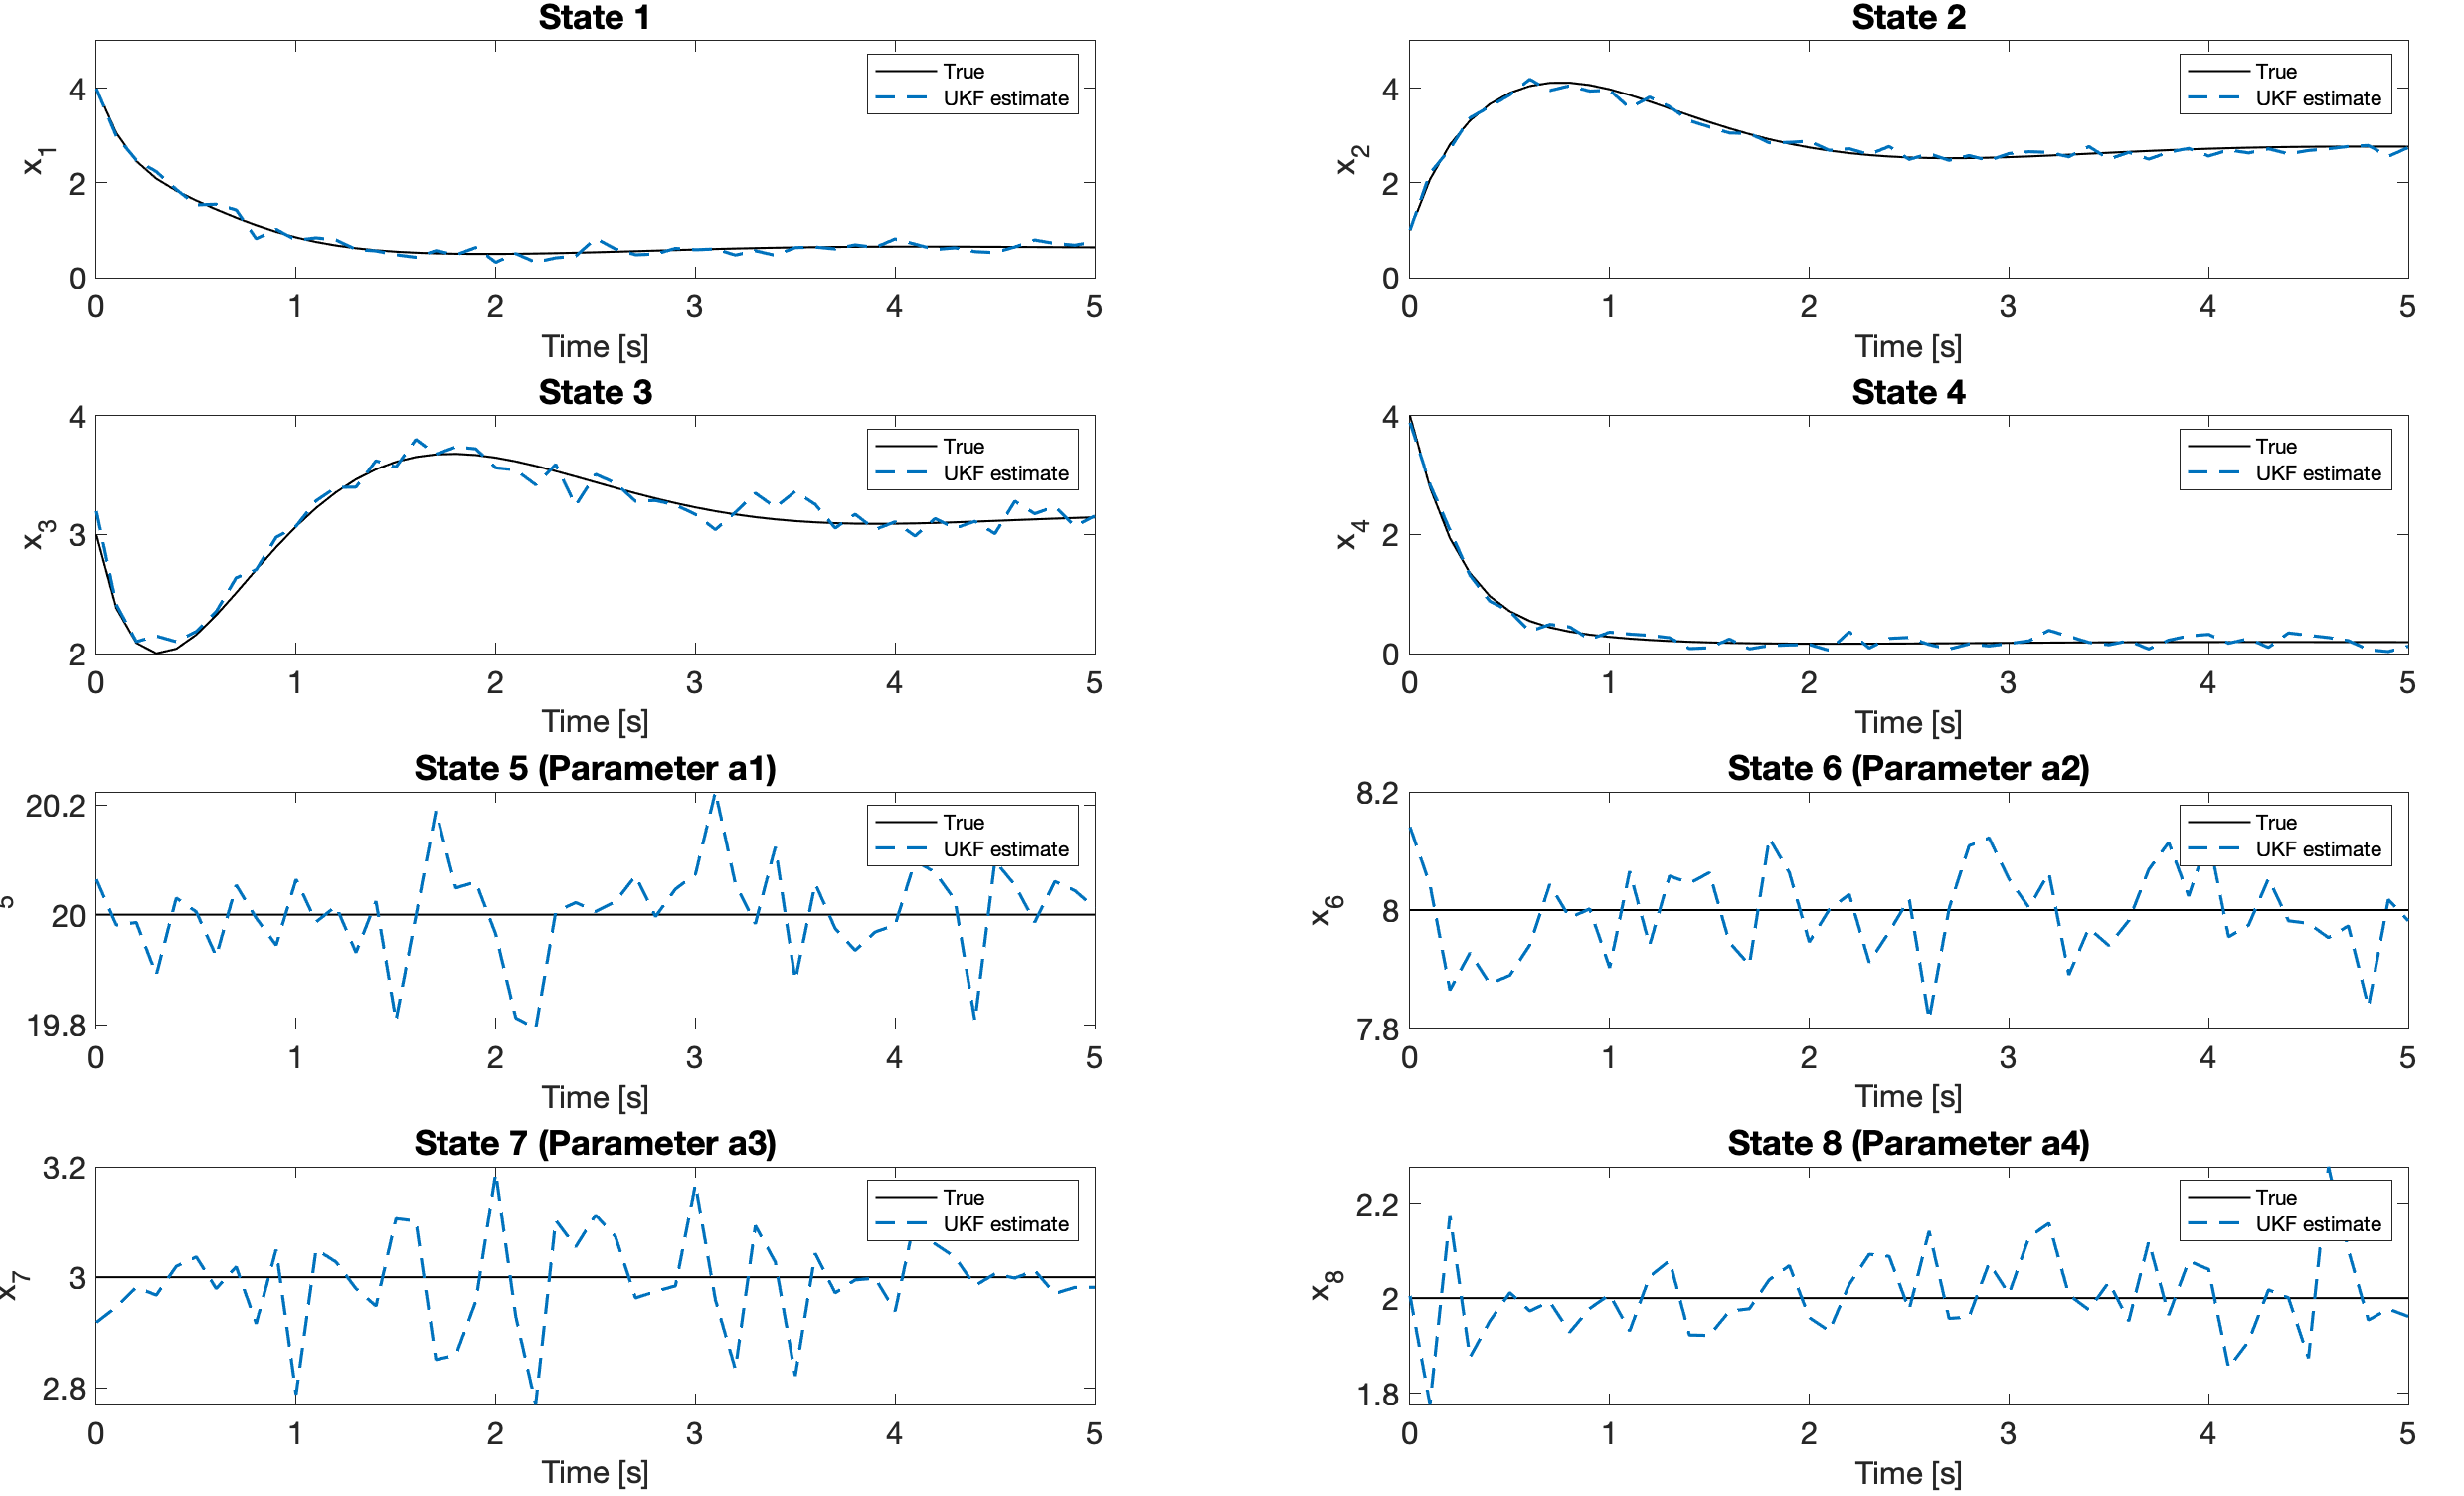
\includegraphics[scale = 0.5]{UKF_4param.png}
    \caption{ds}
    \label{fig:UKF_4param}
\end{figure}

\begin{center}
\begin{table}[h]
\centering
\begin{tabular}{ |P{2cm}||P{1cm} P{2.5cm} P{2.5cm} P{2.5cm} |}
    \hline
    \multicolumn{5}{|c|}{Parameter Values} \\ 
    \hline
     Parameters & True & EKF estimate & UKF estimate &IUKF estimate \\
    \hline
    $\alpha_1$ & 20.0  & 20.0125 &20.0125&19.9744 \\
    $\alpha_2$ & 8.0  & 7.9819  &7.9819& 8.0017 \\
    $\alpha_3$ & 3.0  & 2.9818 &2.9818& 3.0015 \\
    $\alpha_4$ & 2.0 & 1.9614 &1.9614 & 2.0016 \\
    \hline
\end{tabular}
\caption{This table shows the true values of the parameters, the final EKF prediction of the parameters (as a reference to compare filter performance), the final UKF prediction of parameters, and the final IUKF prediction of the parameters. Here, the term final is being used to denote the performance of the filter after 50 time-steps. Interestingly, the performance of the EKF is the exact same as the performance of the UKF. By changing the hyper-parameters for the UKF, the model may be able to provide more accurate results.}
\label{tab:UKF_4param}
\end{table}
\end{center}

\clearpage

\clearpage
\noindent Residuals, also known as the innovation, are one way to access the model's performance. Recall that the residual is the difference between the actual measurement values and the predicted measurement values. Generally, a strong residual graph has

\begin{itemize}
\item a symmetrical distribution that is clustered toward the center,
\item values that are close to 0,
\item a random or unclear pattern.
\end{itemize}

\noindent Figure ~\ref{fig:4params} is the residual graph of the system where the EKF is applied to the four states and four parameters, $\alpha_1, \hdots, \alpha_4$. While this residual graph has values close to 0 and a symmetrical distribution, the pattern is similar to the behavior of the states. Therefore, though UKF can be applied to this nonlinear system, performance can be further optimized.

\begin{figure}[h]
    \centering
    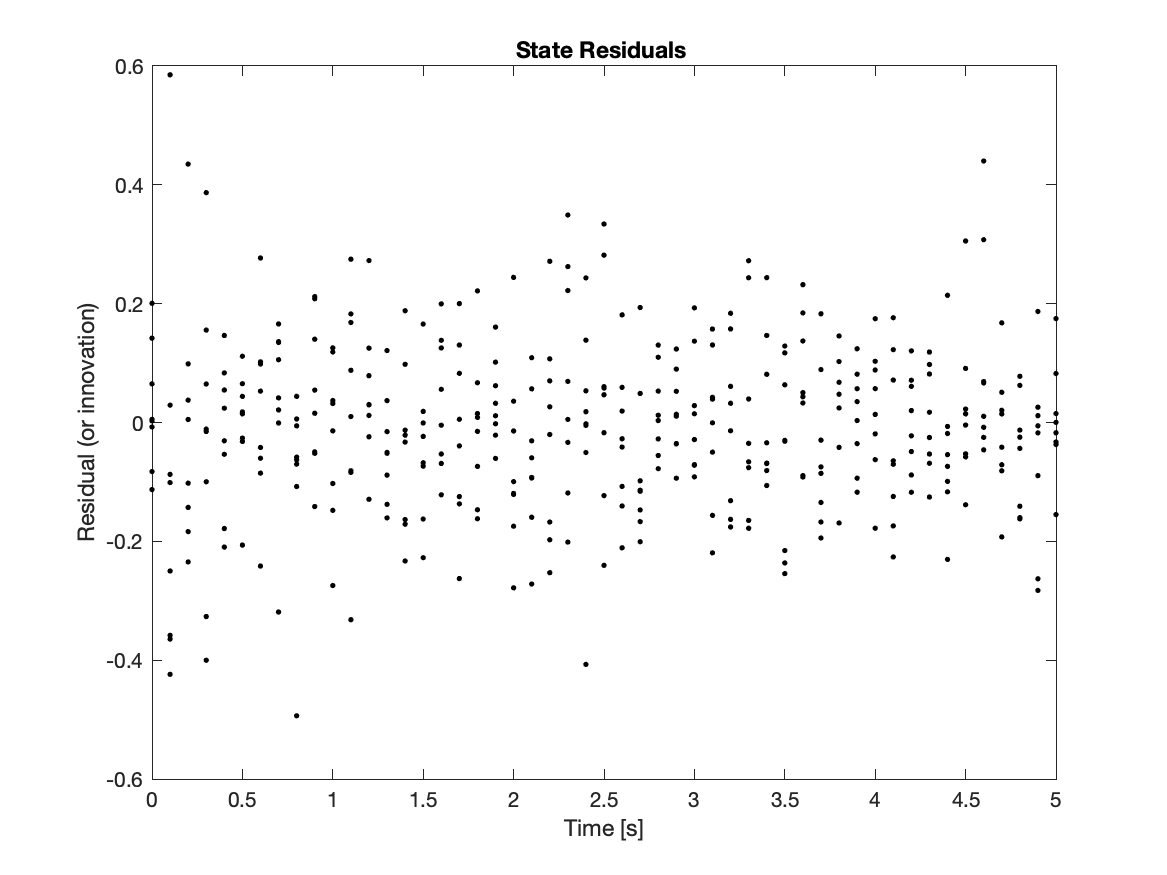
\includegraphics[scale = 0.6]{UKF_4param_residual.png}
    \caption{Built in matlab, four state correction and 4 param}
    \label{fig:4params}
\end{figure}

\noindent Future work includes using the UKF for parameter fitting. One approach would be to use a technique similar to the one employed in chapter 3.2. Alternatively, another non-linear Kalman Filter technique, known as the Dual Unscented Kalman Filter, may also be a promising solution. Either of these two methods will likely be better than the method used in chapter 3.2, because calculating the exponential matrix and jacobian of the system is very computationally expensive and can be avoided with the UKF.

%\noindent \textcolor{red}{Expand here on correcting for 1+ states, currently we are having technical challenges in completing this step}















\chapter{Future Work}
\label{Future Work}


This thesis was inspired by previous work that involved modeling a system that forecasted glucose in real time in patients with Type 2 Diabetes. Researchers utilized the Dual Unscented Kalman Filter for simultaneous state and parameter estimation \cite{article1}. The goal of this thesis was to create a similar model for Type 1 Diabetes (T1D). In previous work by \cite{Shtylla}, a 12 state mathematical model for T1D was developed. The relationship between these 12 states are shown in Figure ~\ref{fig:relations}

\begin{figure}[h]
    \centering
    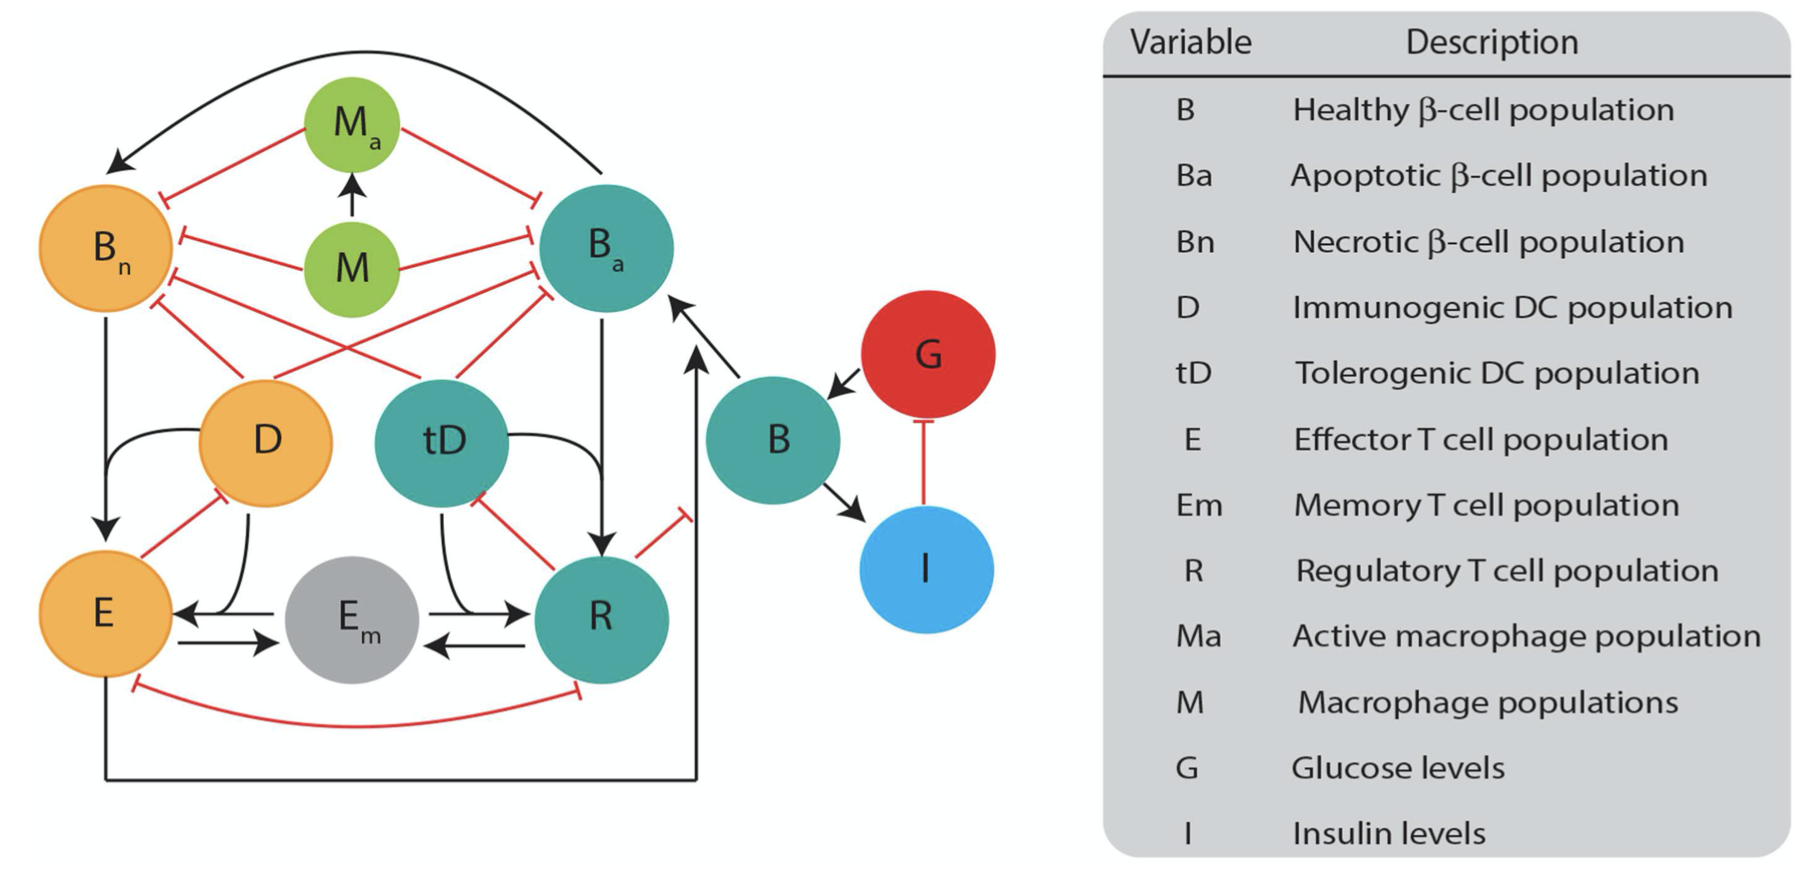
\includegraphics[scale = 0.5]{t1d_model.png}
    \caption{This image is taken from \cite{Shtylla} and provides a visualization on the relationships between the 12 states in this Type 1 Diabetes system.}
    \label{fig:relations}
\end{figure}

The 12 state system is given as 
\begin{align*}
    &\frac{d}{dt} G = R_0 - (G_0 + S_I I)G \\ 
    &\frac{d}{dt}  I = \sigma_1 K_1 (G, G_1) B - \delta_1 I \\
    &\frac{d}{dt} M = J +(k+b)M_a -cM - f_M MB_a - f_M MB_n - e_1M(M+M_a) \\
    & \frac{d}{dt} M_a = f_M MB_a +f_M MB_n - kM_a - e_2M_a(M + M_a) \\
    &\frac{d}{dt} B = \alpha_B K_1(G)B - \delta_B B - \eta_e(t)K_2(E,R)B - W(B, t)\\
    & \frac{d}{dt} B_a = \Tilde{\delta_B} + \Tilde{\eta_e} (t)K_2(E,R)B + \Tilde{W}(B, t) \\
    & \quad \quad  \quad \quad - dB_a - f_M MB_a - f_{M_a} B_a - f^{tD}(D_{SS} - D)B_a - f_D DB_a \\
    &\frac{d}{dt} B_n = dB_a - f_M MB_n - f_{M_a} M_a B_n - F_{Td}(D_{SS} - D)B_n - f_D DB_n \\
    & \frac{d}{dt} D = f_{tD}B_n(D_{SS} - D - tD) + f_{tD}B_n tD - b_{DE} ED - \mu_D D \\
    & \frac{d}{dt} tD = f_{tD}B_a(D_{SS} - D - tD) - f_{tD}B_n tD - b_{IR}RtD - \mu_D tD \\
    & \frac{d}{dt} E = a_E (T_{naive} - E) + b_p \frac{DE}{\theta_D + D} - r_{am}E + b_EDE_m - \mu_E ER \\
    & \frac{d}{dt} R = a_R (T_{naive} - R) + b_p \frac{tDR}{\theta_D + tD} - r_{am}R + b_R tDEm - \mu_R ER, \\
    & \frac{d}{dt} Em = r_{am}(E + R) - (a_{Em} + b_E D + b_R tD)eM
\end{align*}

\noindent \\ \\
\noindent Future direction includes utilizing parameter estimation techniques from this thesis and applying them to this system. Since this system has several more dimensions and is more complex than other systems considered in this thesis, results using the UKF will likely be better than that of the EKF. In addition, further study of alternative parameter estimation techniques, especially the Dual Unscented Kalman Filter, can be beneficial. \\ \\



\chapter{Conclusion}
\label{Conclusion}

\noindent In all, this thesis explored the theory of the KF, EKF, and UKF while also applying the EKF and UKF in both state and joint parameter estimation. Recall from Chapter ~\ref{chap:two} that applying any version of the KF depends on converting systems into their state space format. Chapter ~\ref{chap:three} explores how the KF can be applied to linear dynamical systems while Chapter ~\ref{Extended Kalman Filters} and Chapter ~\ref{Unscented Kalman Filters} explores the EKF and UKF, respectively, as nonlinear forms of the KF. The EKF and UKF each use different ways to linearize the system. Since the EKF linearizes around a single point, utilizing the EKF in complex and high dimensional systems can be ineffective. However, the metabolites example given in Chapter ~\ref{Extended Kalman Filters} has only 4 states and is not highly complex, yielding strong performance in state estimation. The UKF addresses the shortcomings of the EKF by linearizing around multiple points instead of just one. When applying the UKF to the metabolites example, the UKF state estimation had a strange anomaly in State 3, while the other states converged quickly. \\

\noindent The applications of the EKF and UKF in parameter estimation was an important aspect of this research. This thesis utilized joint parameter estimation, which declares an unknown parameter as a separate state to be estimated. It was expected that the UKF would perform better than the EKF because the UKF has a more accurate linearization technique. However, when applied to the metabolites example, performance of the EKF is roughly the same as the performance of the UKF. Tuning the $\alpha, \beta$ and $\kappa$ hyper-parameters of the UKF is likely to yield better results. Future directions for parameter estimation includes looking into alternative methods of parameter estimation. While this thesis only explored joint state estimation, there is a separate dual approach to parameter estimation. In addition, exploration of the Dual Unscented Kalman Filter (DUKF) may be promising. The DUKF was adapted from the UKF and is used to simultaneously estimate states and parameters. \\

\noindent The results of the examples explored in this thesis are overly optimistic and may not reflect model performance of real world systems. This is mainly due to the way the model is initialized. Recall the Van der Pol oscillator from Chapter ~\ref{Unscented Kalman Filters}, where it was observed how the initial state guess, process noise values, and measurement noise values largely influence model performance and convergence. All of the examples in the thesis are initialized with values close to the system's true values and assume low values of measurement and process noise, which are factors that aid faster convergence. In addition, all of the parameter estimation examples operate with the assumption that all states and parameters are measurable--which is not an assumption that should be made of all real world systems. \\ 

\noindent Future directions of this work includes applying the methods explored in this thesis to real world examples, such as the Type 1 Diabetes model. The Type 1 Diabetes model is highly complex and contains 12 states, making this system more complex than the examples considered in this thesis. Furthermore, this model will not be using simulated data; therefore, system measurements will likely be more variable and less predictable. In all, the KF, EKF, and UKF are useful state and parameter estimation methods that can greatly aid in mathematical modeling.

\bibliographystyle{plain}
\bibliography{bib.bib}




\appendix
\lstset{language=Matlab,%
    %basicstyle=\color{red},
    breaklines=true,%
    morekeywords={matlab2tikz},
    keywordstyle=\color{blue},%
    morekeywords=[2]{1}, keywordstyle=[2]{\color{black}},
    identifierstyle=\color{black},%
    stringstyle=\color{mylilas},
    commentstyle=\color{mygreen},%
    showstringspaces=false,%without this there will be a symbol in the places where there is a space
    numbers=left,%
    numberstyle={\tiny \color{black}},% size of the numbers
    numbersep=9pt, % this defines how far the numbers are from the text
    emph=[1]{for,end,break},emphstyle=[1]\color{red}, %some words to emphasise
    %emph=[2]{word1,word2}, emphstyle=[2]{style},    
}


\chapter{Van Der Pol Code}
\label{Van Der Pol Code}\





\newpage
\chapter{Meskin Code}
\label{Meskin Code}
\section{Main function}
\lstinputlisting{Meskin.m}

\newpage
\chapter{Albers Code}
\label{Albers Code}


\end{document}
